\documentclass[specialist, subf, href, colorlinks=true, 14pt, final]{disser}
\usepackage[a4paper, mag=1000, includefoot, left=3cm, right=1.5cm, top=2cm, bottom=2cm, headsep=1cm, footskip=1cm]{geometry}

\usepackage[T2A]{fontenc}
\usepackage [utf8] {inputenc}
\usepackage[english, russian]{babel}
\usepackage{caption}
\usepackage{enumerate}
\usepackage{amsmath,amsthm,amssymb}
\usepackage{wrapfig}
\usepackage{makecell}
%\usepackage {enumitem}  
%\usepackage{graphicx}
%\usepackage{multicol}
\usepackage{multirow}
\usepackage{mathrsfs}
\usepackage{xcolor}
\usepackage{tikz}
\usetikzlibrary{decorations.pathreplacing}
\setcounter{tocdepth}{2}
%\usepackage{hyperref}
%\usepackage{algorithm}
%\usepackage[noend]{algpseudocode}
%\usepackage[margin=1in]{geometry}

\theoremstyle{definition}
\newtheorem{defn}{Определение}[section]
\newtheorem{example}{Пример}[section]
\newtheorem{state}{Утверждение}[section]
\newtheorem{theorem}{Теорема}[section]
\newtheorem{lemma}{Лемма}[section]
\newtheorem{axiom}{Аксиома}[section]
\newtheorem{consequence}{Следствие}[section]

\newcommand{\RNumb}[1]{\uppercase\expandafter{\romannumeral #1\relax}}

\newcommand{\anonsection}[1]{\section*{#1}\addcontentsline{toc}{section}{#1}}
\newcommand{\anonsubsection}[1]{\subsection*{#1}\addcontentsline{toc}{subsection}{#1}}
\newcommand{\pdfrac}[2]{\frac{\partial #1}{\partial #2}}
\newcommand{\const}{\text{const}}
\newcommand{\tang}{\text{tg}}
\newcommand{\npart}[2]{\noindent #1. \underline{#2}}
  
 % Цвета для гиперссылок
\hypersetup{pdfstartview=FitH, linkcolor=blue, urlcolor=blue, colorlinks=true}


\begin{document}

\begin{titlepage}
\begin{center}
МОСКОВСКИЙ ГОСУДАРСТВЕННЫЙ УНИВЕРСИТЕТ\\
имени М. В. Ломоносова\\
Механико-математический факультет\\
\vspace{1cm}
\begin{figure}[!htp]%
  \begin{center}%
        {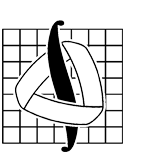
\includegraphics[width=20mm]{pics/mmlogo.png}}%
  \end{center}
\end{figure}
\vspace{4cm}
\Large{
ЗАДАЧИ ФИЗИКО-МЕХАНИЧЕСКОГО ПРАКТИКУМА ПО ГАЗОВОЙ И ВОЛНОВОЙ ДИНАМИКЕ
}\\
\vspace{4cm}
\end{center}
\end{titlepage}

\tableofcontents

\anonsection{Раздел 1}
\anonsubsection{Задача 1. Продольное соударение упругих стержней}
Целью работы является изучение процесса соударения двух стержней и определение скорости упругой волны и деформации, возникающей в стержнях при ударе.\\
I. \underline{Описание явления}\\
Процесс распространения малых возмущений в изотропной 
упругой среде в общем случае можно изучать, исследуя решения 
уравнений Ляме для конкретных начальных и граничных условий [I]. 
Однако общая задача о распространении волн в ограниченном упругом
пространстве довольно сложна. Сен-Венаном разработана 
приближенная теория продольных волн в длинных тонких стержнях. При этом в
качестве основного предположения принята гипотеза плоских 
сечений, т.е. полагается, что любое плоское сечение, образованное
точками среды и перпендикулярное оси стержня, остается при 
движении плоским и перпендикулярным оси, а напряжение во всех 
точках такого сечения одинаково и меняется только со временем. 
Принятые предположения позволяют рассматривать продольное движение
стержней в одномерной постановке.\\
II. \underline{Теоретическая часть}\\
Рассмотрим соударение двух стержней с равной начальной 
длиной $l_0$ , изготовленных из одного и того же материала и имеющих
одинаковое начальное поперечное сечение $S_0$ (Рис. \ref{1-1-1}).
Пусть недеформированный стержень I движется вдоль своей оси
со скоростью $v_0$ и в момент $t = 0$ касается соосного с ним 
стержня II. Для изучения последующего процесса соударения введем 
неподвижную ось $Ox$ с началом, совпадающим с левым торцом первого
стержня в момент $t = 0$.\\
\begin{figure}[!htp]
  \center{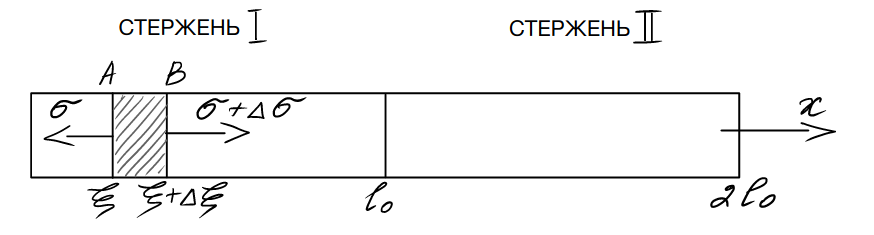
\includegraphics[width=160mm]{pics/1-1-1.png}}
  \caption{}
  \label{1-1-1}
\end{figure}
\\
В качестве лагранжевой координаты рассмотрим начальную 
координату сечения $\xi = x(0)$. Перемещение $u = u(\xi, t)$ можно 
представить в виде
\[
  u(\xi, t) = x(\xi, t) - \xi
\]
Тогда скорость $v$ и продольная деформация $\varepsilon$ в данном сечении $\xi$ соответственно равны
\begin{equation}\label{eq111}
  v = \frac{\partial u}{\partial t},\ \ \varepsilon = \frac{\partial u}{\partial \xi}
\end{equation}
Запишем уравнение движения (второй закон Ньютона) для 
выделенного малого элемента AB (Рис. \ref{1-1-1}), ограниченного сечениями $\xi$ и $\xi + \Delta\xi$:
\begin{equation}\label{eq112}
  \rho\Delta\xi S_{0} \frac{\partial v}{\partial t} = S_{0} \left[\sigma(\xi+\Delta\xi, t) - \sigma(\xi, t)\right],
\end{equation}
где $\rho$ -- начальная плотность материала стержней; $\sigma(\xi,t)$ -- напряжение в данном сечении $\xi$. 
Поделив (\ref{eq112}) на $\Delta\xi$ и сделав предельный переход $(\Delta\xi \rightarrow 0)$, приходим к уравнению
\begin{equation}\label{eq113}
  \rho\frac{\partial v}{\partial t} = \frac{\partial \sigma}{\partial \xi}
\end{equation}
Материал стержней считаем линейно-упругим, т.е.
\begin{equation}\label{eq114}
  \sigma = E\varepsilon,
\end{equation}
где $Е$ - модуль Юнга. 
Уравнения (\ref{eq111}), (\ref{eq113}), (\ref{eq114}) позволяют написать замкнутую систему уравнений для определения скорости и деформации:
\begin{equation}\label{eq115}
  \begin{aligned}
  &\pdfrac{v}{t} = a_{0}^{2} \pdfrac{\varepsilon}{\xi},\\ 
  &\pdfrac{v}{\xi} = \pdfrac{\varepsilon}{t}
  \end{aligned}
\end{equation}
где $a_{0}^{2} = \sqrt{E/\rho}$.
В начальный момент времени $(t = 0)$ первый стержень 
напряжен и имеет скорость $v$, а второй стержень покоится, т.е.
\begin{equation}\label{eq116}
  \begin{aligned}
  &\text{при } t = 0,\ 0 \leqslant \xi < l_{0};\ \varepsilon = 0,\ v = v_{0};\\ 
  &\text{при } t = 0,\ l_{0} < \xi \leqslant 2l_{0};\ \varepsilon = 0,\ v = 0.
  \end{aligned}
\end{equation}
На свободных торцах стержней во всё время движения напряжение равно нулю, поэтому при $t > 0$
\begin{equation}\label{eq117}
  \varepsilon(0, t) = \varepsilon(2l_{0}, t) = 0
\end{equation}
В месте контакта стержней $(\xi = l_{0})$ должны быть равны скорости
и напряжения, т.е. при $t > 0$
\begin{equation}\label{eq118}
  \varepsilon(l_{0}^{-}, t) =\varepsilon(l_{0}^{+}, t),\ \ v(l_{0}^{-}, t) = v(l_{0}^{+}, t)
\end{equation}
Здесь знаки $(-)$, $(+)$ соответствуют значениям функции при подходе слева и справа к точке $\xi = l_0$. Для решения системы (\ref{eq115}) приведем ее к характеристическому виду [\ref{eq112}, \ref{eq113}]. Для этого первое уравнение системы умножим на $dt$, второе -- на $d\xi$ и сложим полученные равенства:
\[
  \pdfrac{v}{t}dt + \pdfrac{v}{\xi}d\xi = a_{0}^{2}\pdfrac{\varepsilon}{\xi}dt + \pdfrac{\varepsilon}{t}d\xi
\]
Левая часть данного уравнения является полным дифференциалом $dv$ для любых $(dt, d\xi)$. Найдем характеристические направления $d\xi = \lambda dt$ такие, вдоль которых и правая часть полученного уравнения является полным дифференциалом. Легко видеть, что таких направлений два $d\xi = \pm a_{0}dt$ в каждой точке фазовой плоскости $(\xi, t)$. \\
Таким образом, мы имеем уравнения характеристик и соотношений на них:
\begin{equation}\label{eq119}
  d\xi = \pm a_{0}dt,\ \ \ dv = \pm a_{0}d\varepsilon
\end{equation}
Полученные соотношения позволяют решить поставленную условиями (\ref{eq116})-(\ref{eq118}) граничную задачу.\\
\begin{figure}[!htp]
  \center{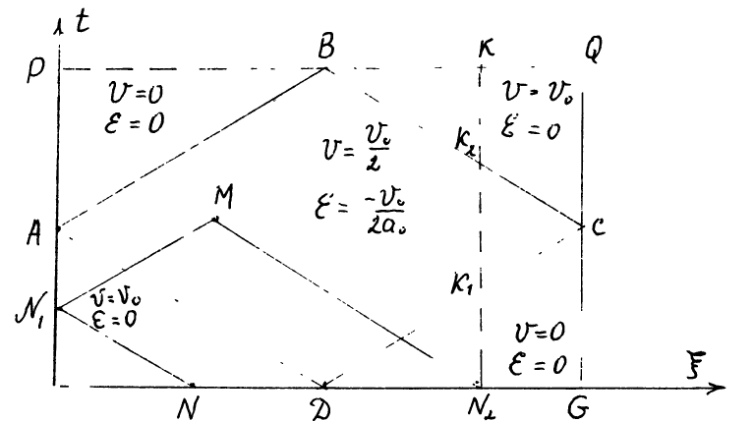
\includegraphics[width=160mm]{pics/1-1-2.png}}
  \caption{}
  \label{1-1-2}
\end{figure}
\\
Покажем это на примере определения решения в точке $M$ (Рис. \ref{1-1-2}). Линии $MN_1$, $MN_2$, $N_{1}N$ являются характеристиками. Сначала определяем решение в граничной точке $N_1$, затем в точке $M$.\\
Из условия (\ref{eq119}) на характеристике $NN_1$ после интегрирования
и использования начальных условий (\ref{eq116}) в точке $N$ получаем $v = -a_{0}\varepsilon + v$. Это уравнение выполняется в любой точке характеристики $NN_1$ и содержит два неизвестных. В точке $N_1$, помимо данного уравнения, должно быть выполнено граничное условие (\ref{eq117}), т.е. в точке $N_1$ мы получили два уравнения для определения скорости и деформации, откуда находим
\begin{equation}\label{eq1110}
  v = v_{0},\ \ \varepsilon = 0.
\end{equation}
Аналогично получаем:
\begin{equation}\label{eq1111}
  \begin{aligned}
  &\text{на характеристике } N_{1}M:\ \ v = a_{0}\varepsilon + v_{0};\\
  &\text{на характеристике } N_{2}M:\ \ v = -a_{0}\varepsilon;
  \end{aligned}
\end{equation}
постоянные интегрирования здесь определены полученным решением в точке $N_1$ (\ref{eq1110}) и начальными условиями (\ref{eq116}) в точке $N_2$ (Рис. \ref{1-1-2}). Из системы (\ref{eq1111}) находим решение в точке $M$: $v = v_{0}/2,\ \varepsilon = -v_{0}/(2a_{0})$. Данный метод решения позволяет определить значения скорости и деформации в любой точке исследуемой области фазовой плоскости. Найденные решения приведены на Рис. \ref{1-1-2}. Область
$OPQG$ разбита характеристиками $AB$, $BC$, $CD$ и $DA$ на пять частей, в каждой из которых решение постоянно. Отметим, что момент времени, соответствующий прямой $PQ$ фазовой плоскости, будет концом соударения,
поскольку в этот момент условия (\ref{eq118}) не выполняются и происходит разлет стержней.\\
Проанализируем полученное решение (Рис. \ref{1-1-2}). В произвольном
сечении $N_{2}K$ второго стержня поведение решения следующее. До 
момента времени, соответствующего точке $K_1$ (момент прихода волны
нагрузки), все параметры сохраняют свои начальные значения. Затем
скачком меняются и остаются постоянными до момента времени, соответствующего точке $K_2$ (момент прихода отраженной от свободного
торца волны разгрузки $CB$). В момент прохождения волны разгрузки параметры решения в данном сечении снова скачком меняются, причем деформация принимает нулевое значение. Данный анализ позволяет сказать, что распространению возмущений в фазовой плоскости соответствуют характеристики. При этом величина $a_0$ является скоростью распространения возмущений но материальным частицам сечений стержня.\\
III. \underline{Экспериментальная часть}\\
Схема экспериментальной установки приведена на Рис. \ref{1-1-3}. 
Плоско-параллельное движение стержней 1 обеспечивается их подвеской на тягах 2. Заданная скорость соударения определяется высотой $h$, с которой сбрасывается стержень
\[
  v_{0} = \sqrt{2gh}
\]
\begin{figure}[!htp]
  \center{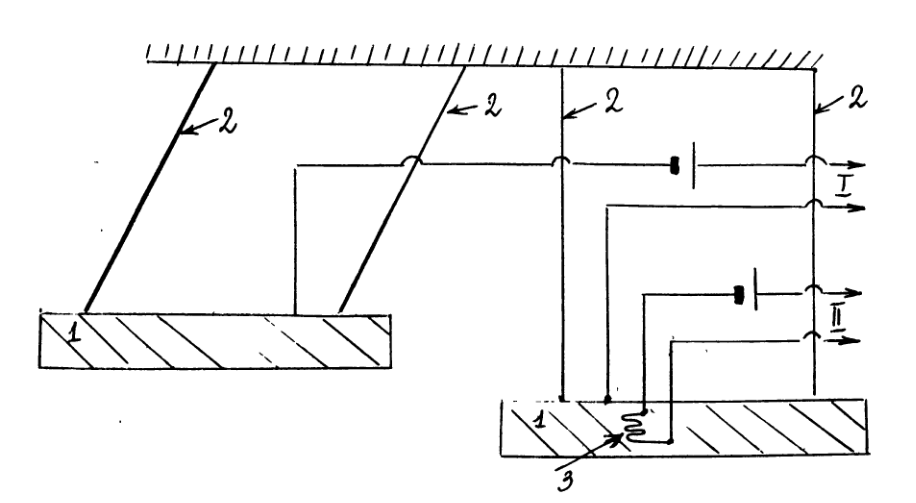
\includegraphics[width=160mm]{pics/1-1-3.png}}
  \caption{}
  \label{1-1-3}
\end{figure}
\\
Эксперимент основан на определении поведения деформации в фиксированном сечении второго стержня, в котором наклеивается тензодатчик 3. В момент касания стержней ($t = 0$) замыкается цепь I запуска развертки осциллографа. На вертикальную развертку осциллографа подается сигнал из цепи II тензодатчика 3. Расстояние от середины тензодатчика до свободного торца второго стержня известно и равно $L$.\\
В результате соударения на экране осциллографа наблюдается сигнал (Рис. \ref{1-1-4}), который фиксируется на фотопленку.\\
\begin{wrapfigure}[7]{l}{0.65\linewidth} 
  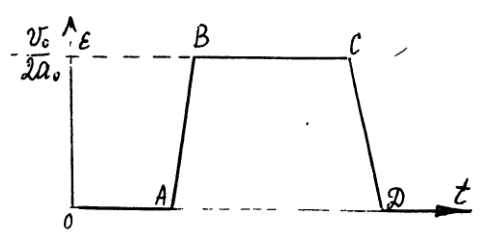
\includegraphics[width=100mm]{pics/1-1-4.png}
  \caption{}
  \label{1-1-4}
\end{wrapfigure}
\\
На Рис. \ref{1-1-4} точка $A$ соответствует времени подхода волны нагрузки к началу тензодатчика, точка $B$ -- времени его полного нагружения. Точки $C$ и $D$ соответствуют началу разгрузки и полной разгрузке датчика отраженной от свободного торца волной. При этом за время $T$, соответствующее длине средней линии трапеции $ABCD$, волна пробегает дважды расстояние $L$ -- от середины датчика до свободного правого торца второго стержня (рис. \ref{1-1-3}). Поэтому экспериментальное значение скорости распространения возмущений 
определяется выражением
\[
  a = \frac{2L}{T}
\]
Высота трапеции $\Omega$ зависит от изменения напряжения в цепи тензодатчика. Изменение напряжения определяется изменением сопротивления датчика в результате его деформации.\\
При линейном усилении сигнала можно считать связь между скачком $\Omega$ и вызывающей этот скачок деформацией линейной, т.е.
\begin{equation}\label{eq1112}
  \varepsilon = k\Omega
\end{equation}
Тензометрический датчик 3 (рис. \ref{1-1-3}) изготовлен из константовой проволоки диаметром 0.03 мм с измерительной базой в 10 мм. Будучи наклеенным на металлический стержень, датчик воспринимает его деформацию. Деформация и изменение сопротивления датчика связаны соотношением
\begin{equation}\label{eq1113}
  \varepsilon = \frac{1}{S}\frac{\Delta R_{g}}{R_{g}}
\end{equation}
где $S$ -- коэффициент тензочувствительности; $R_g$ -- сопротивление недеформированного датчика; $\Delta R_{g}$ -- изменение сопротивления датчика в результате его деформации. Для определения коэффициента пропорциональности $k$ в формуле (\ref{eq1112}) проводится тарировка. Во время тарировки сопротивление в цепи датчика меняется на известную величину путем включения дополнительного сопротивления $R_T$ (рис. \ref{1-1-5}).
\begin{figure}[!htp]
  \center{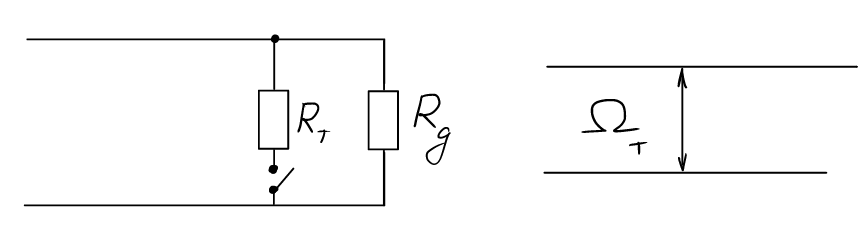
\includegraphics[width=160mm]{pics/1-1-5.png}}
  \caption{}
  \label{1-1-5}
\end{figure}
\\
При включении дополнительного тарировочного сопротивления $R_T$ сопротивление меняется на величину
\begin{equation}\label{eq1114}
  \Delta R_{g} = \frac{R_{g}^{2}}{R_{g} + R_{T}},
\end{equation}
что приводит к скачку $\Omega_{T}$ луча осциллографа. Подставляя изменение сопротивления (\ref{eq1114}) в формулу (\ref{eq1113}), определяем соответствующую данному тарировочному изменению сопротивления деформацию
\[
  \varepsilon_{T} = \frac{R_{g}}{S(R_{g}+R_{T})}
\]
и, учитывая, что $\varepsilon_{T} = k\Omega$, находим из (\ref{eq1112}) экспериментальное
значение деформации
\[
  \varepsilon_{\text{Э}} = \varepsilon_{T}\frac{\Omega}{\Omega_{T}}
\]
\\\\\\
IV. \underline{Порядок выполнения работы}\\
1) В начале работы проводится включение и прогрев осциллографа (согласно инструкции по его эксплуатации). В эксперименте используются два луча. На один из них подается сигнал с датчика, второй луч должен быть установлен на высоте тарировочного скачка первого луча. Поэтому в начале работы проводится включение в цепь датчика тарировочного сопротивления и на высоте подскока первого луча устанавливается второй луч.\\
2) Осциллограф переводится в режим работы с ждущей разверткой лучей и проверяется его автоматический запуск в момент касания стержней.\\
3) Стержень 1 отводится назад, тем самым обеспечивается заданная высота подъема.\\
4) Приводится в готовность фотоаппарат. Фотоаппарат устанавливается на произвольную выдержку.\\
5) Работающий на осциллографе нажимает кнопку фотоаппарата и подает команду на сброс стержня. Фиксация заканчивается после удара.\\
6) Опыт повторяется для других высот подъема стержня.\\
\\
V. \underline{Требования к отчёту}\\
Отчет оформляется и виде заполненной таблицы обработки осциллограмм и проведенных экспериментов и сравнения экспериментальных значений деформации и скорости звука с их теоретическими значениями.
\begin{center}
\begin{tabular}{|c|c|c|c|c|c|c|c|c|c|c|c|}
\hline
N &$h$, мм&$v_0$, м/с&$\Omega$, мм&$\Omega_T$, мм& $\varepsilon_T$ & $\varepsilon_{\text{Э}}$ & $\varepsilon$ & $T$, с & $L$, м & $\frac{\varepsilon_{\text{Э}} - \varepsilon}{\varepsilon}$ & $\frac{a - a_{0}}{a_{0}}$\\
\hline
1 &  &  &  &  &  &  &  & &  &  &\\
\hline
2 &  &  &  &  &  &  &  & &  &  &\\
\hline
\end{tabular}
\end{center}
При этом теоретическое значение деформации определяется решением (рис. \ref{1-1-2}).\\
\\
VI. \underline{Упражнения}\\
1) Определить значение деформации в полубесконечном стержне при его ударе о жесткую преграду, если параметры материала стержня $E, \rho$ известны и известна скорость соударения $v_0$.\\
2) Определить коэффициент тензочувствительности $S$ в формуле (\ref{eq1113}) для датчика, представляющего собой цилиндрическую проволоку длиной $l_0$ и радиусом $r_0$ с известными удельным сопротивлением и коэффициентом Пуассона $\nu$ материала проволоки.\\
3) Определить, пользуясь найденным решением (рис. \ref{1-1-2}), закон движения произвольного сечения.\\
\\
VII. \underline{Контрольные вопросы}\\
1) Какие условия на контактной поверхности возникают при соударении стержней из разных материалов?\\
2) Определить погрешность при определении скорости звука $a$, если считать, что погрешность измерения длины равна 1 мм, а погрешность определения времени $10^{-6}$ с.\\
$L = 144.5$ см; $S = 2.9$ -- коэффициент тензочувствительности;\\
$R_{T} = 3000000$ Ом; $R_{g} = 200$ Ом;\\
$t_{\text{разв}} = 200$ мкс/см; $a_{0} = 5100$ м/с -- теоретическое.\\
\begin{center}
ЛИТЕРАТУРА
\end{center}
1. Седов Л.И. Механика сплошной среды. Т.1,2. М.: Наука, 1970.\\
2. Рахматулин Х.А., Демьянов Ю.А. Прочность при интенсивных кратковременных нагрузках. М.: Физматгиз, 1961.\\
3. Гольдсмит В. Удар. М.: Стройиздат, 1965.\\

\anonsubsection{Задача 2. Сверхзвуковое обтекание клина}
%\setcounter{equation}{0}
Целью работы является определение связи между параметрами набегающего потока и параметрами потока, проходящего через косой скачок, возникающий при обтекании тел сверхзвуковым потоком, ознакомление с принципиальной схемой к устройством сверхзвуковой аэродинамической трубы, определение параметров потока в рабочей части трубы по параметрам торможения, а также графическое (методом годографа) решение задачи об обтекании клина сверхзвуковым потоком.\\
I. \underline{Теоретическая часть}\\
1. Если в горизонтальном потоке газа плотностью $\rho$ и скоростью $v$ выделить трубку тока площадью поперечного сечения $\sigma$,
то энергия, переносимая газом массой $m = \rho v \sigma$ через это сечение за секунду складывается из кинетической энергии $mv^{2} / 2$, 
работы сил давления $p \sigma v$ и внутренней энергии $mU$ ($U$ -- внутренняя энергия единицы массы, потенциальная энергия сил тяжести
не учитывается). Полная энергия для единицы массы будет равна
($\rho$ -- плотность):
\addtocounter{equation}{1}
\begin{equation}\label{eq:121}
  E_{e} = \frac{v^2}{2} + U + \frac{p}{\rho}
  \tag{1}
\end{equation}
Уравнение состояния для газа запишется в виде
\addtocounter{equation}{1}
\begin{equation}\label{eq:122}
  p = \rho R T
  \tag{2}
\end{equation}
где $R = C_{p}-C_{v}$; $C_{p}$, $C_{v}$ -- теплоемкости газа при постоянном давлении и постоянном объеме. Для воздуха $R = 288.7\  \text{м}^{2}/\text{с}^{2}\cdot \text{град}$. Величина $U+ p/\rho = C_{p}T = i$ называется теплосодержанием. Учитывая уравнение \eqref{eq:122}, получим
\[
  i = C_{p}\frac{p}{\rho R} = C_{p}\frac{p}{\rho(C_{p}-C{v})} = \frac{p}{\rho}\frac{k}{k - 1}
\]
Здесь $k = C_{p}/C_{v}$ -- показатель адиабаты, для воздуха $k = 1.4$.
Теперь энергию единичной массы газа запишем в виде
\addtocounter{equation}{1}
\begin{equation}\label{eq:121d}
  E_{e} = \frac{v^2}{2} + \frac{k}{k-1}\frac{p}{\rho}
  \tag{1$'$}
\end{equation}
При установившемся течении без вязкости и теплообмена поток энергии вдоль трубки тока сохраняется, поэтому при переходе частицы газа из состояния с параметрами $p_{1},\ \rho_{1},\ v_{1}$ в состояние с 
параметрами $p_{2},\ \rho_{2},\ v_{2}$ выполняется равенство
\addtocounter{equation}{1}
\begin{equation}\label{eq:121dd}
  \frac{v_{1}^{2}}{2}+\frac{k}{k-1}\frac{p_1}{\rho_1} = \frac{v_{2}^{2}}{2}+\frac{k}{k-1}\frac{p_2}{\rho_2}\ \ \text{или}\ \ \frac{v^{2}}{2}+\frac{k}{k-1}\frac{p}{\rho} = \const
  \tag{1$''$}
\end{equation}
Обратим внимание на следующее: если для движущейся частицы газа со скоростью $v$ ее параметры состояния есть давление $p$, плотность $\rho$ и температура $T$, то при адиабатическом (без теплообмена с окружающей средой) торможении до $v = 0$ получим параметры торможения частицы -- давление торможения $p_0$, плотность торможения $\rho_0$ и температуру торможения $T_0$, удовлетворяющие уравнению состояния
\addtocounter{equation}{1}
\begin{equation}\label{eq:122d}
  p_{0} = \rho_{0} R T_{0}
  \tag{2$'$}
\end{equation}
Соответствующие формулы для скорости распространения малых  возмущений или скорости звука будут иметь вид
\addtocounter{equation}{1}
\begin{equation}\label{eq:123}
  a = \sqrt{\frac{dp}{d\rho}} = \sqrt{k\frac{p}{\rho}}\ \ \text{или}\ \ a^{2} = k\frac{p}{\rho} = kRT
  \tag{3}
\end{equation}
\addtocounter{equation}{1}
\begin{equation}\label{eq:123d}
  a_{0} = \sqrt{\frac{dp_{0}}{d\rho_{0}}} = \sqrt{k\frac{p_{0}}{\rho_{0}}}\ \ \text{или}\ \ a_{0}^{2} = k\frac{p_{0}}{\rho_{0}} = kRT_{0}
  \tag{3$'$}
\end{equation}
Для теплосодержания справедливо равенство
\addtocounter{equation}{1}
\begin{equation}\label{eq:124}
  i_{0} = i + v^{2}/2
  \tag{4}
\end{equation}
где $i$ -- теплосодержание частицы единичной массы газа, движущейся со скоростью $v$, a $i_{0} = C_{p}T_{0}$ -- теплосодержание заторможенной частицы (теплосодержание торможения).\\
Из равенства \eqref{eq:124} видно, что при адиабатическом расширении
газа (например, при истечении из сосуда через любой насадок)
скорость расширения (истечения) максимальна при минимальном 
теплосодержании, т.е. когда $i = 0$,
\addtocounter{equation}{1}
\begin{equation}\label{eq:125}
  i_{0} = v_{\text{max}}^{2}/2
  \tag{5}
\end{equation}
В этом случае теплосодержание частицы газа переходит полностью
в ее кинетическую энергию.\\
Далее имеем
\[
  \frac{v^2}{2} = i_{0} - i = C_{p}(T_{0} - T);\ \ \frac{i_{0} - i}{2} = \frac{v^2}{2i}
\]
или
\[
  \frac{T_{0}-T}{T} = \frac{v^2}{2C_{p}T}\cdot\frac{R}{R} = \frac{v^{2}(C_{p}-C-{v})}{2TRC_p} = \frac{k-1}{2}M^{2},
\]
где $M = v/a$ -- число Маха.\\
Итак,
\addtocounter{equation}{1}
\begin{equation}\label{eq:126}
  \frac{T_{0}-T}{T} = \frac{k-1}{2}M^{2}\ \ \text{или}\ \ \frac{T_0}{T} = 1 + \frac{k-1}{2}M^{2}
  \tag{6}
\end{equation}
Если скорость потока (истечения) в некотором месте (сечении канала) равна скорости звука в том же сечении, то такая скорость называется критической. При этом $v_{\text{кр}} = a_{\text{кр}}M = 1$ и формула \eqref{eq:126} примет вид
\addtocounter{equation}{1}
\begin{equation}\label{eq:127}
  T_{0}/T_{\text{кр}} = (k+1)/2\ \ \text{или}\ \ T_{\text{кр}} = 2T_{0}/(k+1)
  \tag{7}
\end{equation}
Отсюда имеем
\addtocounter{equation}{1}
\begin{equation}\label{eq:128}
  a_{0}/a_{\text{кр}} = \sqrt{T_{0}/T_{\text{кр}}} = \sqrt{(k+1)/2}
  \tag{8}
\end{equation}
Для воздуха $k = 1.4$; $R = 29.27$; $g = 9.81$ м/с$^2$, поэтому
\addtocounter{equation}{1}
\begin{equation}\label{eq:129}
  a_{0} = \sqrt{kRT_0} = 20.1\sqrt{T_0};\ \ a_{\text{кр}} = a_{0}\sqrt{\frac{2}{k+1}} = 18.3\sqrt{T_0} 
  \tag{9}
\end{equation}
К этому можно добавить, что 
\addtocounter{equation}{1}
\begin{equation}\label{eq:1210}
  v_{\text{max}} = 2.23a_{0} = 44.8\sqrt{T_0}
  \tag{10}
\end{equation}
Это вытекает из
\[
  \frac{T_{0}-T}{T_{0}} = \frac{v^2}{kRT_0}\frac{k-1}{2} = \frac{k-1}{2}\frac{v^2}{a_{0}^{2}}
\]
при $T\rightarrow 0,\ v\rightarrow v_{\text{max}}$, т.е.
\[
  1 = \frac{v_{\text{max}}^{2}}{a_{0}^{2}}\frac{k-1}{2},\ \ v_{\text{max}} = a_{0}\sqrt{5} \approx 2.23a_0
\]
\\
2. Рассмотрим вопрос об обтекании клина сверхзвуковым потоком газа.
\begin{wrapfigure}[7]{l}{0.6\linewidth} 
  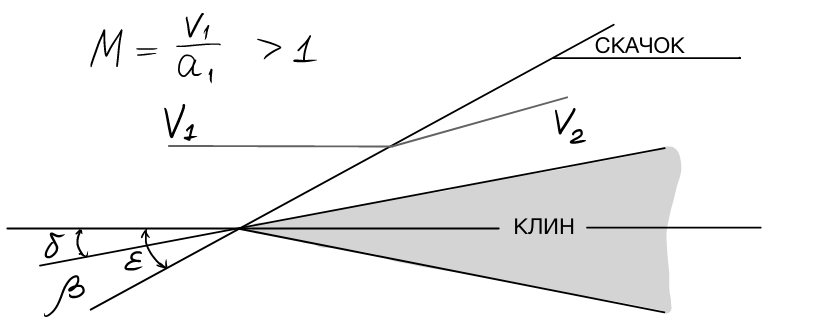
\includegraphics[width=100mm]{pics/1-2-1.png}
  \caption{}
  \label{1-2-1}
\end{wrapfigure}
Теоретическое рассмотрение и опыт показывают, что при натекании на клин с углом при вершине $2\delta$ сверхзвукового потока с числом Маха $M = v_{1}/a_{1} > 1$ к кромке клина присоединяется плоский косой скачок (ударная волна) с наклоном к направлению потока под некоторым углом $\varepsilon$ или под углом $\beta$ по отношению к поверхности клина. При этом поток газа, проходя через косой скачок, поворачивается на угол $\delta$ и идет параллельно поверхности клина [1].\\
Законы сохранения массы, энергии, а также теорема об изменении количества движения позволяют рассчитать все параметры об изменении количества движения потока за скачком, если известны параметры до скачка и угол клина. Обратимся к рис. \ref{1-2-2}.\\
\newpage
Пусть однородный сверхзвуковой поток со скоростью $v_1$ натекает на плоский косой скачок $l-l$, поворачивается на угол $\delta$ и течет за скачком со скоростью $v_2$.\\
\begin{wrapfigure}[9]{l}{0.65\linewidth} 
  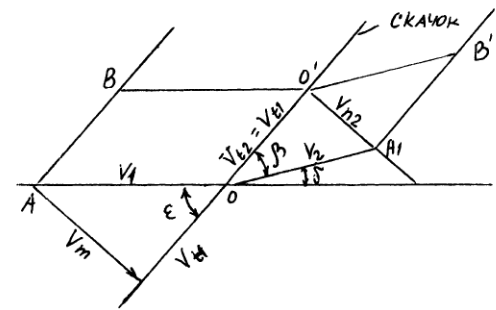
\includegraphics[width=100mm]{pics/1-2-2.png}
  \caption{}
  \label{1-2-2}
\end{wrapfigure}
$v_{n_1},\ v_{t_1},\ v_{n_2},\ v_{t_2}$ -- составляющие скоростей $v_1$ и $v_2$ по нормали к скачку и вдоль него; $p_{1},\ \rho_{1},\ T_{1}$ -- параметры состояния газе до скачка; $p_{2},\ \rho_{2},\ T_{2}$ -- те же параметры состояния газа после скачка. За единицу времени материальная частица, занимавшая объем с боковым сечением $AOO'B$ займет с боковым сечением $OA'B'O'$. Так как перетекание через плоскость скачка может происходить только за счет нормальной составляющем скорости, то уравнение неразрывности в рассматриваемом случае имеет вид
\addtocounter{equation}{1}
\begin{equation}\label{eq:1211}
  \rho_{1}v_{n_1} = \rho_{2}v_{n_2}
  \tag{11}
\end{equation}
На основании теоремы об изменении количества движения для направлений вдоль скачка и перпендикулярно к нему имеем
\addtocounter{equation}{1}
\begin{equation}\label{eq:1212}
  \rho_{1}v_{n_1}v_{t_1} = \rho_{2}v_{n_2}v_{t_2},
  \tag{12}
\end{equation}
и
\addtocounter{equation}{1}
\begin{equation}\label{eq:1213}
  p_{1} + \rho_{1}v_{n_1}^{2} = p_{2} + \rho_{2}v_{n_2}^{2}
  \tag{13}
\end{equation}
Полная энергия частицы до скачка и после него одинакова, поэтому уравнение \eqref{eq:121dd} примет вид
\addtocounter{equation}{1}
\begin{equation}\label{eq:1214}
  \frac{k}{k-1}\frac{p_1}{\rho_1} + \frac{1}{2}v_{1}^{2} = \frac{k}{k-1}\frac{p_2}{\rho_2} + \frac{1}{2}v_{2}^{2}
  \tag{14}
\end{equation}
Если учесть, что $v/a = M,\ a = \sqrt{kp/\rho}$, получим следующие  соотношения между составляющими скоростей и углами, указанными на рис. \ref{1-2-1} и \ref{1-2-2}:
\addtocounter{equation}{1}
\begin{equation}\label{eq:1215}
  \begin{cases}
  v_{1}^{2} = v_{n_1}^{2} + v_{t_1}^{2} = k\frac{p_1}{\rho_1}M_{1}^{2}\\
  v_{2}^{2} = v_{n_2}^{2} + v_{t_2}^{2} = k\frac{p_2}{\rho_2}M_{2}^{2}
  \end{cases}
  \tag{15}
\end{equation}
\addtocounter{equation}{1}
\begin{equation}\label{eq:1216}
  \begin{aligned}
  v_{n_1} = v_{1}\sin\varepsilon,\ \ v_{t_1} = v_{1}\cos\varepsilon\\
  v_{n_2} = v_{2}\sin\beta,\ \ v_{t_2} = v_{2}\cos\beta
  \end{aligned}
  \tag{16}
\end{equation}
Из уравнения \eqref{eq:1212} с учетом равенства \eqref{eq:1211} имеем
\addtocounter{equation}{1}
\begin{equation}\label{eq:1217}
  v_{t_1} = v_{t_2}
  \tag{17}
\end{equation}
а из схемы на рис. \ref{1-2-2}
\addtocounter{equation}{1}
\begin{equation}\label{eq:1218}
  v_{1}/v_{2} = \cos\beta/\cos\varepsilon
  \tag{18}
\end{equation}
Путем ряда преобразование можно получить следующие выражения (см. [1]):
\addtocounter{equation}{1}
\begin{equation}\label{eq:1219}
  p_{2}/p_{1} = \frac{2k}{k+1}\left(M_{1}\sin^{2}\varepsilon - \frac{k-1}{2k}\right),
  \tag{19}
\end{equation}
\addtocounter{equation}{1}
\begin{equation}\label{eq:1220}
  \rho_{1}/\rho_{2} = \frac{2k}{k+1}\left(\frac{1}{M_{1}^{2}\sin^{2}\varepsilon} + \frac{k-1}{2}\right),
  \tag{20}
\end{equation}
\addtocounter{equation}{1}
\begin{equation}\label{eq:1221}
  \tang\varepsilon/\tang\beta = \frac{2}{k+1}\left(\frac{1}{M_{2}^{2}\sin^{2}\beta} + \frac{k-1}{2}\right),
  \tag{21}
\end{equation}
\addtocounter{equation}{1}
\begin{equation}\label{eq:1222}
  \frac{1}{\tang\delta} = \frac{k+1}{2}\left(\frac{M_{1}^{2}}{M_{1}^{2}\sin^{2}\varepsilon - 1} - 1\right)\tang\varepsilon,
  \tag{22}
\end{equation}
\addtocounter{equation}{1}
\begin{equation}\label{eq:1223}
  \varepsilon = \delta + \beta.
  \tag{23}
\end{equation}
Если параметры перед скачком $p_{1},\ \rho_{1},\ M_{1}$ и угол
клина $\delta$ (или $P_2$), то выражения \eqref{eq:1219}-\eqref{eq:1222} дают возможность определить параметры потока за скачком и угол наклона скачка.\\
II. \underline{Графическое решение задачи}\\
Учитывая, что $V_{t_1} = V_{t_2}$, можно картину скоростей перед и за
скачком стационарного потока газа, текущего вдоль оси $Ox$ и набегающего на клин с углом полураствора $\delta$, представить так, как указано на рис. \ref{1-2-3}.
\begin{figure}[!htp]
  \center{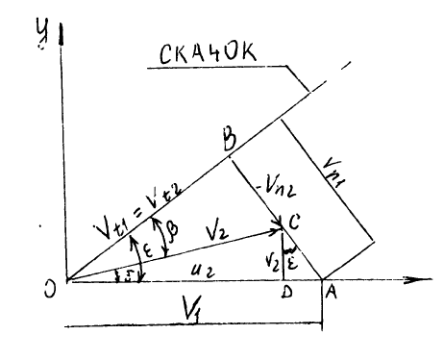
\includegraphics[width=140mm]{pics/1-2-3.png}}
  \caption{}
  \label{1-2-3}
\end{figure}
\\
Здесь по-прежнему индекс 1 соответствует параметрам потока до скачка, индекс 2 -- параметрам потока после скачка, $\delta$ -- угол поворота потока, $\varepsilon$ -- угол наклона скачка к направлению потока. Итак: $OA = V_{1}$, $OB\perp BA$ и $OB = V_{t_1} = V_{t_2}$, $BA = V_{n_1}$, точка С расположена $BA$, $OC = V_2$, $BC = V_{n_2}$, $u_{2},\ v_{2}$ -- проекции скорости $V_2$ на оси $Ox$ и $Oy$ соответственно.\\
Поставим себе целью найти уравнение, связывающее составляющие $u_{2},\ v_{2}$ с параметрами потока до скачка, например в виде $v_{2} = f(u_{2}, V_{1}, V_{\text{кр}})$.\\
Из уравнений \eqref{eq:1211} и \eqref{eq:1213} получаем
\[
  p_{2}-p_{1} = \rho_{1}V_{1}(V_{n_1}-V_{n_2}),
\]
или с учетом подобия треугольников $OBA$ и $DCA$
\addtocounter{equation}{1}
\begin{equation}\label{eq:1224}
  p_{2} = p_{1} + \rho_{1}V_{1}(V_{1}-u_{2}),
  \tag{24}
\end{equation}
Уравнение энергии \eqref{eq:1214} может быть записано в виде
\[
  \frac{k}{k-1}\frac{p_1}{\rho_1} + \frac{1}{2}V_{1}^{2} = \frac{k}{k-1}\frac{p_{0}}{\rho_0}
\]
он из \eqref{eq:129}
\[
  V_{\text{кр}}^{2} = a_{0}\frac{2}{k+1} = kRT_{0}\frac{2}{k+1} = \frac{2k}{k+1}\frac{p_0}{\rho_0},
\]
т.е.
\[
  p_{0}/\rho_{0} = \frac{k+1}{2k}V_{\text{кр}}^{2}
\]
поэтому
\addtocounter{equation}{1}
\begin{equation}\label{eq:1225}
  p_{1} = \rho_{1}\left(V_{\text{кр}}^{2}\frac{k+1}{2k} - V_{1}^{2}\frac{k-1}{2k}\right),
  \tag{25}
\end{equation}
аналогично
\addtocounter{equation}{1}
\begin{equation}\label{eq:1226}
  p_{2} = \rho_{2}\left(V_{\text{кр}}^{2}\frac{k+1}{2k} - V_{2}^{2}\frac{k-1}{2k}\right) = \rho_{2}\left(\frac{k+1}{2k}V_{\text{кр}}^{2} - \frac{k-1}{2k}(u^{2}+v^{2})\right),
  \tag{26}
\end{equation}
Кроме того, из указанного подобия треугольников и условия $\rho_{1}V_{n_1} = \rho_{2}V_{n_2}$ следует
\addtocounter{equation}{1}
\begin{equation}\label{eq:1227}
  \frac{\rho_1}{\rho_2} = \frac{V_{n_1}}{V_{n_2}} = \frac{V_{1}(V_{1} - u_{2})}{u_{2}(V_{1}-u_{2})-V_{2}^{2}}
  \tag{27}
\end{equation}
В самом деле, на основании подобия треугольников $OBA$ и $DCA$
\[
  V_{n_1}/V_{1} = (V_{1} - u_{2})/(V_{n_1} - V_{n_2})
\]
или
\[
\begin{aligned}
  \frac{V_{n_1}}{V_{n_2}} = \frac{V_{1}(V_{1}-u_{2})}{V_{n_1}V_{n_2} - V_{n_2}^{2}} = \frac{V_{1}(V_{1}-u_{2})}{V_{n_1}V_{n_2} - V_{2}^{2} + V_{1}^{2} - V_{n_1}^{2}} = \\
  = \frac{V_{1}(V_{1}-u_{2})}{V_{1}^{2} - V_{n_1}(V_{n_1}-V_{n_2}) - V_{2}^{2}} = \frac{V_{1}(V_{1}-u_{2})}{u_{2}(V_{1}-u_{2}) - V_{2}^{2}}
\end{aligned}
\]
Подставляя значения $p_{1},\ p_{2},\ \rho_{1},\ \rho_{2}$ из \eqref{eq:1226} - \eqref{eq:1227} в \eqref{eq:1224} получим уравнение в виде $f(u_{2}, v_{2}, V_{1}, V_{\text{кр}}) = 0$, дающее связь между составляющими скорости $u_{2}$ и $v_2$ за скачком и содержащее в виде параметра скорость потока $V_1$ перед скачком. Значения величин $V_{\text{кр}}$ и $k$, отражающих состав газа и его начальную температуру торможения, можно считать заданными. Разрешая это уравнение относительно $v_{2}^{2}$, получим
\addtocounter{equation}{1}
\begin{equation}\label{eq:1228}
  v_{2}^{2} = (V_{1}-u_{2})^{2} \frac{u_{2} - V_{\text{кр}}^{2}/V_{1}}{V_{\text{кр}}^{2}/V_{1} + \frac{2}{k+1}V_{1} - u_{2}}
  \tag{28}
\end{equation}
При определенных значениях $k$ и $V_{\text{кр}}$ для каждого значения скорости $V_1$ в плоскости годографа $(u, v)$ зависимость \eqref{eq:1228} представляет собой кривую второго порошка, определяющую геометрическое место точек концов вектора $V_2$. Эта симметричная относительно оси $Ou$ кривая называется строфоидой или угарной полярной. Откладываем на оси $Ou$ отрезки $OD = V_{\text{кр}}^{2}/V_{1}$, $OA = V_1$, $DE = 2V_{1}/(k+1)$. На отрезках $DA$ и $DE$ строим две окружности. Если из произвольной точки $F$ окружности $DFE$ провести прямую $FD$, то она пересечет малую окружность в точке, $H$. Опуская перпендикуляр $FC$ и проводя прямую $AH$, найдем точку  пересечения $B$, которая и будет концом вектора $V_2$, а $OC$ и $BC$ составляющими $u_2$ и $v_2$. Аналогично находятся точки 1, 2, 3, 4.\\
Докажем это. Из построения рис. \ref{1-2-4} вытекает $CF^{2} = DC\cdot CE$ и\\
$CB/CA = CD/CF$ или $CB^{2} = CA^{2}\cdot CD^{2} / CF^{2} = CA^{2}\cdot CD/CE$,\\
но $CA = V_{1}-u_{2}$,\ \ $CD=OC-OD=OC-V_{\text{кр}}/V_{1}$,\\
$CE=OD+DE-OC = V_{\text{кр}}^{2}/2 + 2V_{1}/(k+1)-OC$,\\
поэтому
\addtocounter{equation}{1}
\begin{equation}\label{eq:1228d}
  CB^{2} = (V_{1}-OC)^{2} \frac{OC - V_{\text{кр}}^{2}/V_{1}}{V_{\text{кр}}^{2}/V_{1} + 2V_{1}/(k+1) - OC}
  \tag{28$'$}
\end{equation}

\begin{figure}[!htp]
  \center{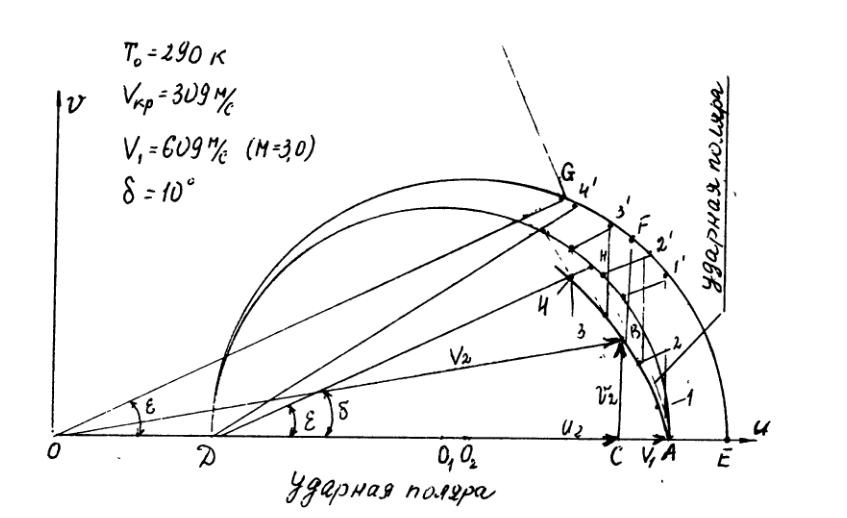
\includegraphics[width=170mm]{pics/1-2-4.png}}
  \caption{}
  \label{1-2-4}
\end{figure}

Если $CB = V_2$, а $OC = u_2$, то \eqref{eq:1228d} совпадает  \eqref{eq:1228}. При перемещении точки $F$ вдоль полуокружности $DFE$ точка $B$ опишет верхнюю половину ударной поляры 1-2-3-4 ... Ударная поляра пересекает ось $Ou$ в точках $D$ и $A$, причем точка $D$ соответствует минимальной скорости $V_{n_2}=V_{\text{кр}}^{2}/V_{1}$, соответствующей скорости потока, проходящего через прямой скачок уплотнения без изменения направления скорости. Точка $A$ является двойной, для нее $V_{2} = V_{1}$, т.е. скачок отсутствует. Участки кривой, лежащие между $u = V_1$ и асимптотой $u = V_{\text{кр}}^{2}/V_{1} + 2V_{1}/(k+1)$, соответствуют $V_{2}>V_{1}$, физического смысла они не имеют.\\
Для практических вычислений часто бывает удобнее пользоваться не скоростью $V$, а числом $M = V/a$ ($a$ -- скорость звука). В этом случае удобнее пользоваться для графического представления уравнением \eqref{eq:1228}, если все его члены разделить на $a_{1}^{2}$:
{\Large
\[
  \frac{v_{2}^{2}}{a_{1}^{2}} = \left(M_{1}-\frac{u_{2}}{a_{1}}\right)^{2}\frac{\frac{u_2}{a_1} - \frac{V_{\text{кр}}^{2}/a_{1}^{2}}{M_1}}{\frac{V_{\text{кр}}^{2}/a_{1}^{2}}{M_1} + \frac{2}{k+1}M_{1} - \frac{u_2}{a_1}}
\]
}

Вид рис. \ref{1-2-4} при этом не изменится, а соответствующие отрезки могут быть выражены через числа $M$: отрезок $OA$ представляет собой число $M_1$, отрезок $OB$ в том же масштабе представляет собой $M_{2}a_{2}/a_{1}$, а отрезки $GA$ и $GB$ выражают собой $M_{n_1}$ и $M_{n_2}a_{2}/a_{1}$. Здесь $a_1$ и $a_2$ -- скорости звука до скачка и за ним. Отношение этих скоростей можно определить по отрезкам $GA$ и $GB$, пользуясь уравнением \eqref{eq:1214}, которое при делении на $a_{1}^{2}$ принимает вид
\[
  \frac{2}{k-1} + M_{n_1}^{2} = \frac{2}{k-1}\cdot\frac{a_{2}^{2}}{a_{1}^{2}} + M_{n_2}\frac{a_{2}^{2}}{a_{1}^{2}}
\]
где учтено, что $V_{t_1} = V_{t_2}$, $a_{1}^{2} = k p_{1}/\rho_{1}$, $a_{2}^{2} = k p_{2}/\rho_{2}$. Заменяя $M_{n_1}$ и $M_{n_2}$ отрезками $GA$ и $GB$, получим
\[
  \frac{2}{k-1} + GA^{2} = \frac{2}{k-1}\cdot\frac{a_{2}^{2}}{a_{1}^{2}} + GB^{2}
\]
или
\[ 
  \frac{a_{2}^{2}}{a_{1}^{2}} = \frac{k-1}{2}(GA^{2} - GB^{2}) + 1.
\]
Отношение плотностей при переходе через скачок равно
\[
  \frac{\rho_1}{\rho_2} = \frac{V_{n_1}}{V_{n_2}} = \frac{GB}{GA}\cdot\frac{a_1}{a_2}
\]
а отношение давлений
\[
  \frac{p_2}{p_1} = \frac{\rho_2}{\rho_1}\cdot\frac{a_{2}^{2}}{a_{1}^{2}} = \left[ \frac{k-1}{2}(GA^{2}-GB^{2})+1\right] \frac{GA}{GB}\cdot\frac{a_1}{a_2}.
\]
\newpage
\noindent III. \underline{Описание экспериментальной установки}

Получение сверхзвуковой скорости осуществляется в аэродинамической трубе А-8, принципиальная схема которой изображена на рис. \ref{1-2-5}.

Сжатый воздух из газгольдеров практически без теплообмена
(вследствие кратковременности процесса), т.е. адиабатически 
расширяется и через систем трубопровода и задвижек поступает в 
фотокамеру, коробку сверхзвуковых сопловых вставок и рабочую часть.
В рабочей части происходит взаимодействие потока воздуха с 
обтекаемой моделью. Силовое воздействие потока на модель 
воспринимается весами (механическими или тензометрическими). Картина 
обтекания может наблюдаться с использованием различных методов 
визуализации (теневой метод, метод сажемаслянового покрытия, метод
нитей и т.д.). Для использования оптического метода с применением прибора ИАБ-451 в стенках рабочей части монтируются оптически однородные стекла. Спектры обтекания могут наблюдаться на матовом
стекле, фотографироваться или сниматься на киноленту.

\noindent IV. \underline{Порядок выполнения и оформления задачи}

1) Совместно с оператором подготовить аэродинамическую трубу к экспериментальной работе и провести эксперимент: поставить модель клина в рабочую часть аэродинамической трубы, закрыть все двери и люки контура трубы, подготовить прибор ИАБ-451, установить фотокамеру АФА или матовое стекло, открыть задвижку Лудло, при помощи быстродействующей задвижки выйти на заданный режим, снять отсчеты печатающим механизмом, сфотографировать спектр обтекания.

2) Пользуясь данными протокола печатающего механизма, величиной давления и температурой атмосферы и описанием задачи, построить ударную поляру и составить таблицу параметров сверхзвукового обтекания клина.\\
\begin{figure}[!htp]
  \center{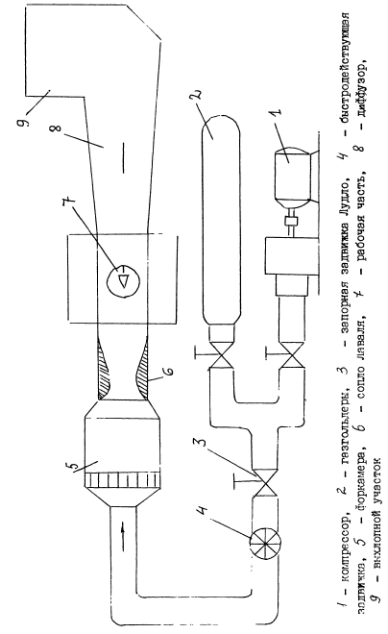
\includegraphics[width=150mm]{pics/1-2-5.png}}
  \caption{}
  \label{1-2-5}
\end{figure}

Таблица заполняется в следующей последовательности:
\begin{enumerate}
  \item снимаются показания барометра $p_{\text{В}}$ и термометров в помещении $t_{\text{П}}$ и наружи $t_{\text{Н}}$, определяется атмосферное давление\footnote{Давление во всех случаях должно выражаться в одних и тех же единицах};
  \item $p_0$ определяется по показаниям измерителя полного давления;
  \item $T_0$\ \ $t_{\text{Н}}$ + 273 град."К";
  \item $\rho_0$ определяется по формуле \eqref{eq:122};
  \item $a_0$ определяется по формуле \eqref{eq:123} или \eqref{eq:129};
  \item $V_{\text{кр}}$ определяется по формуле \eqref{eq:129};
  \item $p_1$ определяется по показаниям измерителя статического давления;
  \item $M_1$ определяется по таблицам как функция отношения $p_{0}/p_{1}$;
  \item $\rho_{1},\ a_{1}$ определяются но таблицам при полученном значении $V_1$;
  \item $V_{1} = M_{1}a_{1}$
  \item $V_{2y},\ M_{2y}$ определяется по ударной поляре;
  \item $\varepsilon_{y}$ определяется по ударной поляре;
  \item $\varepsilon_{c}$ определяется по спектру обтекания;
  \item {\large$\Delta\varepsilon = \frac{\varepsilon_{c}-\varepsilon{y}}{\varepsilon_{c}}\cdot 100\%$};
  \item $\gamma$ определяется по спектру (угол между линией Маха за скачком и поверхностью клина);
  \item {\large $M_{2c} = 1/\sin\gamma$,\ \ $\Delta M_{2} = \frac{M_{2c}-M_{2y}}{M_{2c}}\cdot 100\%$.}\\
\end{enumerate}

\begin{center}
ТАБЛИЦА ДАННЫХ ДЛЯ ВЫПОЛНЕНИЯ ЗАДАЧИ:\\
$p_{\text{В}} = $\ \ \ \ \ \ \ \ мм рт.ст., \ \ 
$t_{\text{П}} = $\ \ \ \ \ \ \ \ град. C,\\
$p_{\text{атм}} = $\ \ \ \ \ \ \ \ кг/см$^2$, \ \ 
$t_{\text{Н}} = $\ \ \ \ \ \ \ \ град. C\\

\vspace{0.5cm}
\begin{tabular}{|l|p{4cm}|p{4cm}|p{4cm}|}
\hline
 & \makecell{$\delta = 5^o$} & \makecell{$\delta = 10^o$} & \makecell{$\delta = 15^o$}\\
\hline
 $p_0$, кг/см$^2$ & & &\\
\hline
 $T_0$, град "К" & & &\\
\hline
 $\rho$, кГс$^2\cdot$м$^{-4}$ & & &\\
\hline
 $a_0$, м/с & & &\\
\hline
 $V_{\text{кр}}$, м/с & & &\\
\hline
 $p_1$, кг/см$^2$ & & &\\
\hline
 $\rho_1$, кГс$^2\cdot$м$^{-4}$ & & &\\
\hline
 $a_1$, м/с & & &\\ 
\hline
 $M_1$ & & &\\
\hline
 $V_{1}$, м/с & & &\\ 
\hline
 $V_{2y}$, м/с & & &\\
\hline
 $M_{2y}$ & & &\\
\hline
 $\varepsilon_{y}$, град. & & &\\
\hline
 $\varepsilon_{c}$, град. & & &\\
\hline
 $\Delta\varepsilon$, \%\% & & &\\
\hline
 $\gamma$, град. & & &\\
\hline
 $M_{2c}$ & & &\\
\hline
 $\Delta M_{2}$, \%\% & & &\\
\hline
\end{tabular}
\end{center}
\newpage
\begin{center}
ЛИТЕРАТУРА
\end{center}
1. Черный Г.Г. Газовая динамика. М.: Наука, 1988. С.297-306.\\
2. Ферри А. Аэроданамика сверхзвуковых течений. М.-Л.: ГИТТЛ,
Госиздат технико-теоретической литературы, 1952. С.52-63.\\
3. Рахматулин Х.А., Сагомонян А.Я., Бунимович А.И., Зверев И.Н.
Газовая динамика. М.: Высшая школа, 1965. С.318-326.\\
4. Зауэр Р. Введение в газовую динамику. М.-Л.: ГИТТЛ, 1947.
C.115-120.

\newpage
\anonsubsection{Задача 3. Поперечные колебания бруса}
Целью работы является определение собственных частот и нормальных форм изгибных колебаний стержней, а также определение модуля продольной упругости методом колебаний.

\noindent I. \underline{Описание явления}\\
Нормальные формы и собственные частоты изгибных колебаний бруса

Механическая система с одной степенью свободы, выведенная из состояния равновесия и освобожденная затем от действия внешних сил, может совершать свободные гармонические колебания с определенной частотой, называемой собственной частотой. 

Примером могут служить колебания математического маятника, колебания груза, подвешенного на пружине малой массы и имеющего возможность перемещаться только в вертикальном направлении, крутильные колебания тонкого стержня с массой на конце и т.д.

В последних двух примерах пружина и стержень ввиду их малой массы играют роль только восстанавливающих усилий, упругих связей; возникающими в них инерционными усилиями можно пренебрегать по сравнению с силой инерции груза.

В теоретической механике показано, что механическая система с $n$ степенями свободы имеет $n$ собственных частот, соответствующих $n$ видам нормальных колебаний, так что перемещение каждой точки системы при свободных колебаниях представляется в виде геометрической суммы перемещений, которые получила бы точка при каждом из нормальных колебаний. При одном только нормальном колебании каждая точка системы совершает гармоническое колебание. Таким образом, \underline{нормальным колебанием} материальных точек называется такое свободное движение, при котором каждая точка совершает простое гармоническое колебание, причем частоты колебаний всех точек одинаковы и все точки колеблются в одной фазе.

Упругое тело, рассматриваемое как материальный континуум, имеет бесчисленное множество степеней свободы: каждая точка из бесчисленного множества материальных точек имеет три степени свободы, а взаимодействие ее с другими точками образует упругие связи. Поэтому упругое тело обладает бесчисленным множеством собственных частот, соответствующих бесчисленному множеству нормальных колебаний. Вектор перемещения точек упругого тела при каком-то $n$-ом нормальном колебании $U_n$ представляется, следовательно, таким образом:
{\Large
\[
  \overline{U_n} = \overline{u}(x, y, z) e^{i\omega_{n} t}
\]
}
где $\omega_n$ -- постоянная, определяющая собственную частоту. Из 
этого выражения для $\overline{U_n}$, видно, что форма тела при нормальном колебании изменяется во времени подобно самой себе. Произвольное свободное колебание можно представить в виде суммы нормальных колебаний:
{\Large
\[
  \overline{U}(x,y,z,t) = \sum\limits_{n}\overline{U_n}(x,y,z) e^{i\omega_{n} t}.
\]
}
Возможность представления сложных движений упругого тела при свободных колебаниях в виде результата наложения нормальных колебаний соответствует возможности разложения функции в тригонометрический ряд (теорема Фурье).

Если на упругое тело действует периодическая внешняя нагрузка с частотой, равной одной из собственных частот тела, то имеет место \underline{резонанс} -- амплитуда колебаний тела при отсутствии диссипативных сил будет возрастать теоретически до бесконечности, хотя практически всегда имеются диссипативные силы (внешние и
внутренние), препятствующие безграничному возрастанию амплитуды,
явление резонанса может привести к возникновению недопустимо
больших напряжений и к разрушению, особенно в случае резонанса на одной из низших собственных частот. В других случаях, наоборот, пользуются явлением резонанса для раскачки тел. Отсюда ясно, почему важно определение собственных частот и соответствующих им нормальных форм колебаний упругих тел.\\
\noindent II. \underline{Теоретическая часть}\\
Изгибные колебания бруса

Примем при рассмотрении поперечных колебаний балки за основу гипотезу плоских сечений. При этом, материальные частицы, которые в недеформированном состоянии находились в плоскости ортогонального сечения балки, переходят в результате деформации в плоскость, ортогональную серединному волокну, длина которого не меняется (это волокно называется нейтральным).
\begin{figure}[!htp]
  \center{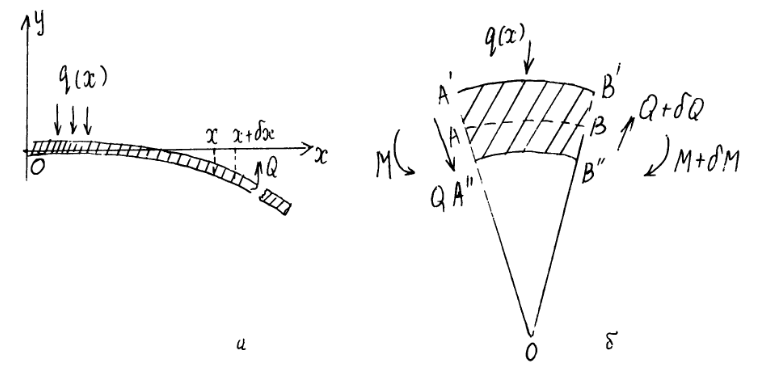
\includegraphics[width=160mm]{pics/1-3-1.png}}
  \caption{}
  \label{1-3-1}
\end{figure}
На рис. \ref{1-3-1} $Q(x)$ -- перерезывающая сила; $M(x)$ -- изгибающий момент; $q(x)$ -- внешняя сила, приходящаяся на единицу длины.

Для равновесия балки необходимо ввести вместо мысленно отброшенной части балки (рис. \ref{1-3-1}, а) некоторую силу $Q$ (перерезывающая сила). Кроме силы $Q$ в сечении действует изгибающий момент $М$ (риc. \ref{1-3-1}, б), обусловленный растягиванием внешних волокон $A'B'$ и сжатием внутренних -- $A''B''$. В силу гипотезы плоских сечений распределение деформаций по толщине балки имеет вид
\addtocounter{equation}{1}
\begin{equation}\label{eq:131}
  \varepsilon(y_{0}) = y_{0}/R
  \tag{1}
\end{equation}
где $y_0$ -- лагранжева координата рассматриваемого волокна, значение $y_{0}=0$ соответствует нейтральному волокну; $R$ -- радиус кривизны нейтрального волокна.

Считая материал балки линейно-упругим $(\sigma = E\varepsilon)$, находим интегрированием по площади поперечного сечения результирующий момент
\addtocounter{equation}{1}
\begin{equation}\label{eq:132}
  M = EJ/R,
  \tag{2}
\end{equation}
где $E$ -- модуль Юнга материала балки; $J = \int\limits_{S}y_{0}^{2}ds$ -- момент инерции сечения балки относительно оси, ортогональной плоскости движения и проходящей через нейтральное волокно.

Величина $EJ$ называется жесткостью балки.

Для равновесия выделенного элемента балки длиной $dx$ должны быть выполнены условия равенства нулю главного вектора сил и моментов:
\addtocounter{equation}{1}
\begin{equation}\label{eq:133}
  \begin{aligned}
  & \delta Q = q(x)\delta x\\
  & Q\delta x = \delta M
  \end{aligned}
  \tag{3}
\end{equation}

Пусть $y(x)$ -- уравнение нейтрального волокна. Для малых прогибов $y'' \approx 1/R$. Тогда из \eqref{eq:133} и \eqref{eq:132} получим уравнение равновесия балки
\addtocounter{equation}{1}
\begin{equation}\label{eq:134}
  EJ\pdfrac{^{4}y}{x^4} = q(x)
  \tag{4}
\end{equation}

В случае свободного движения балки внешними силами являются силы инерции. В этом случае $y=y(x,t)$ т.е. прогиб является функцией времени, а $q(x,t) = -\rho S_{0} \partial^{2}y/\partial t^2$ (при свободных колебаниях согласно принципу Даламбера внешнюю распределенную нагрузку $q(x,t)$ следует заменить силами инерции). С учетом этого из \eqref{eq:134} получаем уравнение свободных колебаний балки
\addtocounter{equation}{1}
\begin{equation}\label{eq:135}
  EJ\pdfrac{^{4}y}{x^4} + \rho S_{0}\pdfrac{^{2}y}{t^2} = 0,
  \tag{5}
\end{equation}
где $S_0$ -- площадь сечения.

Если балка совершает нормальное изгибное колебание, то каждая точка его оси колеблется гармонически, причем частоты колебаний всех точек одинаковы и колебания совершаются в одной фазе, поэтому для обнаружения собственных частот и нормальных форм колебаний ищем частное решение уравнения \eqref{eq:135} в виде
\addtocounter{equation}{1}
\begin{equation}\label{eq:136}
  y(x, t) = e^{i\omega t} Y(x)
  \tag{6}
\end{equation}
где $Y(x)$ -- функция, характеризующая форму собственных колебаний (вид изогнутой оси), $\omega$ -- частота колебаний.

Подстановка \eqref{eq:136} в \eqref{eq:135} приводит к обыкновенному дифференциальному уравнению
\addtocounter{equation}{1}
\begin{equation}\label{eq:137}
  \frac{d^{4}Y(x)}{dx^4} - k^{4}Y(x) = 0,
  \tag{7}
\end{equation}
где
\addtocounter{equation}{1}
\begin{equation}\label{eq:13star}
  k^{4} = \omega^{2}\rho S_{0} / (EJ).
  \tag{*}
\end{equation}

Общим решением этого уравнения является функция
\addtocounter{equation}{1}
\begin{equation}\label{eq:138}
  Y(x) = C_{1}\text{ch}(kx) + C_{2}\text{sh}(kx) + C_{3}\cos (kx) + C_{4}\sin (kx)
  \tag{8}
\end{equation}

Если балка безгранична по длине и имеет опор, то ничего другого о нормальных колебаниях сказать нельзя: никаких ограничений на частоту колебаний $\omega$ не налагается, а нормальная форма колебаний ограничена только видом \eqref{eq:138} при неопределенных коэффициентах $C_{1},\ C_{2},\ C_{3},\ C_{4}$. Следовательно, для такого бруса (балки) любая частота может быть собственной, иначе говоря безграничный брус имеет непрерывный спектр собственных частот.

В брусе конечной длины имеются определенные граничные условия (условия закрепления), которые ограничивают произвол постоянных $C_{1}$, $C_{2}$, $C_{3}$, $C_{4}$; для этих величин получаются из граничных условий линейные однородные алгебраические уравнения, которые содержат в коэффициентах величину $k$, связанную с частотой $\omega$. Из условия наличия нетривиальных решений этой системы уравнений (иначе ни о каких колебаниях говорить нельзя) получается уравнение, вообще говоря трансцендентное, для $\omega$, называемое уравнением частот. Таким образом, наличие границ делает спектр собственных частот дискретным.

Так как из системы однородных уравнений, в коэффициенты которой подставляются корни уравнения частот, определяются только отношения искомых постоянных, например $C_{1} / C_{4}$, $C_{2} / C_{4}$, $C_{3} / C_{4}$, то форма нормального колебания определяется с точностью
до постоянного множителя. Это соответствует тому, что форма изогнутой оси при нормальном колебании изменяется во времени подобно самой себе, причем амплитуда колебаний остается неопределенной.

При разных способах закрепления концов получаются различные уравнения частот и различные формы нормальных колебаний.

Рассмотрим случай, когда балка свободна на одном конце и жестко заделана на другом.

Пусть конец балки $x = 0$ жестко заделан, а конец $x = L$ -- свободен. В заделке прогиб и наклон касательной к изогнутой оси балки равны нулю, т.е.
\addtocounter{equation}{1}
\begin{equation}\label{eq:139}
  y(0, t) = \partial y / \partial x |_{x = 0} = 0.
  \tag{9}
\end{equation}
На другом конце балки равны нулю изгибающий момент и перерезывающая сила, т.е.
\addtocounter{equation}{1}
\begin{equation}\label{eq:1310}
  \begin{aligned}
  Q(L, t) = EJ \partial^{3} y / \partial x^{3} |_{x=L} = 0,\\
  M(L, t) = EJ\partial^{2} y / \partial x^{2} |_{x=L} = 0
  \end{aligned}
  \tag{10}
\end{equation}
Если на свободный торец поместить груз массы $m$, то первое условие в \eqref{eq:1310} заменится уравнением движения груза массы $m$:
\[
  m\pdfrac{^{2}y(L,t)}{t^2} = -Q(L,t),
\]
а второе -- сохранится, если пренебречь инерцией вращения груза.

Граничные условия \eqref{eq:139} и \eqref{eq:1310} позволяют получить для определения постоянных $C_{1}$, $C_{2}$, $C_{3}$, $C_{4}$ систему однородных уравнений
\addtocounter{equation}{1}
\begin{equation}\label{eq:1311}
  \begin{cases}
  C_{1} + C_{3} = 0\\
  C_{2} + C_{4} = 0\\
  C_{1}\text{ch}(kL) + C_{2}\text{sh}(kL) - C_{3}\cos (kL) - C_{4}\sin (kL) = 0\\
  m\omega^{2}[C_{1}\text{ch}(kL) + C_{2}\text{sh}(kL) + C_{3}\cos (kL) + C_{4}\sin (kL)] =\\
  \ \ = k^{3}EJ[C_{1}\text{sh}(kL) + C_{2}\text{ch}(kL) + C_{3}\sin (kL) - C_{4}\cos (kL)]
  \end{cases}
  \tag{11}
\end{equation}
которая имеет нетривиальное решение только в случае равенства нулю ее определителя. Условие равенства нулю определителя и приводит к уравнению частот:
\addtocounter{equation}{1}
\begin{equation}\label{eq:1312}
  m\omega^{2}\left[\text{sh}(kL)\cos(kL) - \text{ch}(kL)\sin (kL)\right] - k^{3}EJ\left[1 + \text{ch}(kL)\cos (kL)\right] = 0.
  \tag{12}
\end{equation}
При отсутствии груза $(m=0)$ уравнение \eqref{eq:1312} имеет вид
\addtocounter{equation}{1}
\begin{equation}\label{eq:1313}
  \text{ch}(kL)\cos (kL) + 1 = 0.
  \tag{13}
\end{equation}
Каждому действительному корню этого уравнения $k_{n}L$ соответствует значение собственной частоты колебаний. Корнями уравнения \eqref{eq:1313} являются
\[
  k_{1}L = 1.875;\ \ k_{2}L = 4.694;\ ... \ ;\ k_{n}L = \frac{2n-1}{2}\pi;\ ...
\]

Принимая во внимание обозначение \eqref{eq:13star}, для собственных 
частот колебаний получаем
\addtocounter{equation}{1}
\begin{equation}\label{eq:1314}
  \omega_{1} = \lambda\left(\frac{1.875}{L}\right)^{2};\ \ \omega_{2} = \lambda\left(\frac{4.694}{L}\right)^{2};\ ...
  \tag{14}
\end{equation}
где $\lambda^{2} = EJ/(\rho S_{0})$.

Из системы уравнений \eqref{eq:1311} для каждого значения $k_{n}L$ можно определить отношение $C_{3}/C_{4}$:
{\large
\[
  \left(\frac{C_3}{C_4}\right)_{n} = -\frac{\text{sh}(k_{n}L) + \sin(k_{n}L)}{\text{ch}(k_{n}L) + \cos(k_{n}L)},
\]
}
так что форма нормальных колебаний определяется с точностью до
постоянного множителя $A_n$:
{\large
\[
  \begin{aligned}
  A_{n}Y_{n}(x) = \left[\text{sh}(k_{n}L) + \sin(k_{n}L)\right]\left[\text{ch}(k_{n}x) - \cos(k_{n}x)\right] - \\
   - \left[\text{ch}(k_{n}L) + \cos(k_{n}L)\right]\left[\text{sh}(k_{n}x) - \sin(k_{n}x)\right].
  \end{aligned}
\]
}

При каждом нормальном колебании имеется некоторое число точек оси, которые остаются неподвижными. Эти точки называются \underline{узлами} колебаний. Те точки между узлами, в которых амплитуда колебаний максимальна, называются \underline{пучностями}. Узел отличается от точки защемления бруса тем, что помещение в узле шарнирной опоры не приведет к возникновению опорной реакции. Поэтому, если положение узлов какой-либо конструкции известно, то удобно точки опоры располагать в узлах: инерционные усилия в этом случае не будут передаваться основанию.

Положение узлов определяется из уравнения $Y_{n}(x) = 0$, т.е. из уравнения
\addtocounter{equation}{1}
\begin{equation}\label{eq:1315}
  \begin{aligned}
  \left[\text{sh}(k_{n}L) + \sin(k_{n}L)\right]\left[\text{ch}(k_{n}x) - \cos(k_{n}x)\right] - &\\
   - \left[\text{ch}(k_{n}L) + \cos(k_{n}L)\right]\left[\text{sh}(k_{n}x) - \sin(k_{n}x)\right] = 0.&
  \end{aligned}
  \tag{15}
\end{equation}
Вид изогнутой оси (нормальная форма) для первых трех нормальных
колебаний показан схематически на рис. \ref{1-3-2}.

При колебаниях с собственной частотой $\omega_{1}$ неподвижной остается только точка закрепления (рис. \ref{1-3-1}, а). При колебаниях с частотой $\omega_2$ имеется один узел (рис. \ref{1-3-1}, б). При колебаниях с частотой $\omega_3$ появятся две узловых точки (рис. \ref{1-3-2}, в). Подсчеты показывают (см., например, [2]), что положения узлов определяются следующими числами, дающими отношение расстояния узла от свободного конца балки к длине балки.

\begin{center}
\begin{tabular}{p{7cm} p{2.5cm} p{2.5cm} p{2.5cm}}
  Порядковый номер\\ нормального колебания & \multicolumn{3}{c}{Положения узлов колебаний} \\
  & 1-й & 2-й & 3-й\\
  I & - & - & -\\
  II & 0.226 & - & -\\
  III & 0.132 & 0.499 & -\\
  IV & 0.094 & 0.356 & 0.6439\\
\end{tabular}
\end{center}
\begin{figure}[!htp]
  \center{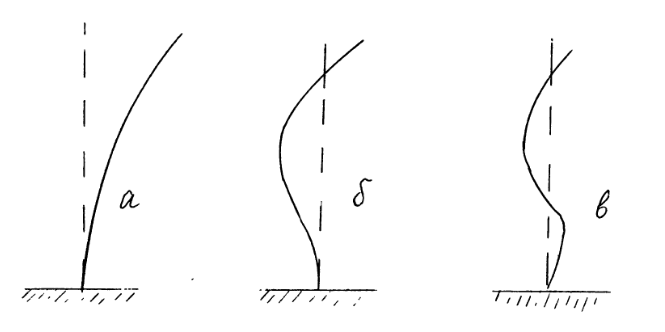
\includegraphics[width=160mm]{pics/1-3-2.png}}
  \caption{}
  \label{1-3-2}
\end{figure}
\newpage
По наличию этих узловых точек можно в опытах судить о том, что брус совершает одно из нормальных колебаний.

\noindent III. \underline{Экспериментальная часть}

1. Описание экспериментальной установки.\\
Балка 1 длины $L$ (рис. \ref{1-3-3}) закреплена вертикально одним
концом в массивной подставке 2. На другом конце балки может быть закреплен груз 3 массой $m$. В некотором сечении балки наклеен постоянный магнит 4. При поперечных колебаниях балки магнит индуцирует ток в индуктивном датчике 5, расположенном на штативе 6. Электрический ток из цепи датчика, возникающий в результате индукции, подается на вход осциллографа. Основной измеряемой величиной является период собственных колебаний. Вблизи защемленного конца расположим электромагнит 7, после чего изменением частоты задающего генератора стандартных частот 8 добиваются совпадения одной из собственных частот колебаний стержня. О наступлении резонанса судят по появлению четко выраженных узлов колебаний и по максимальному возрастанию амплитуды. Форма нормальных колебаний (число узлов) указывает на порядковый номер собственной частоты.

Расстояния узлов от концов стержня измеряются линейкой.
\begin{figure}[!htp]
  \center{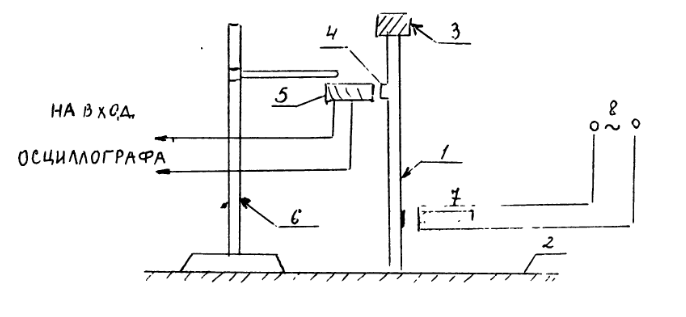
\includegraphics[width=170mm]{pics/1-3-3.png}}
  \caption{}
  \label{1-3-3}
\end{figure}

2. Определение модулей упругости по опытам на колебания\\
Для практических целей является существенно важными опыты по определению собственных частот и форм нормальных колебаний конструкций или их элементов, теоретические расчеты, для которых бывают сложными.

Поскольку теория изгибных колебаний проверена на многих опытах и является надежной, опыты по изгибным колебаниям стержней могут служить также для другой важной цели -- для определения механических характеристик материалов.

Механические характеристики (модули упругости, предел упругости и т.п.) зависят в той или иной мере от скорости деформаций. В опытах на колебания, регулируя частоту вынуждающей силы и амплитуду колебаний, можно в довольно широких пределах изменять скорость деформации.

В формулы для определения собственных частот колебаний 
входят модули упругости материала. В этих формулах собственные 
частоты можно считать известными, поскольку они определены из 
опытов, а искомыми величинами считать значения модулей упругости
при соответствующей скорости деформации. Например, в случае изгибных колебаний по формуле \eqref{eq:13star} находим
\[
  E = \frac{\omega^{2}\rho S_{0}L^{4}}{J(kL)^4}
\]
Если здесь вместо $\omega$ писать измеренную в опыте собственную
частоту $\omega_{n}$, а вместо $kL$ -- соответствующее значение корня уравнения частот, то для значения модуля продольной упругости при этой частоте получим
\addtocounter{equation}{1}
\begin{equation}\label{eq:1316}
  E_{n} = \frac{\omega_{n}^{2}\rho S_{0}L^{4}}{J(k_{n}L)^4}
  \tag{16}
\end{equation}
Для большинства металлов изменение модуля продольной упругости
очень слабо зависит от скорости деформации, так что из опытов
на колебания получают обычно значения $E$, близкие к тем, которые определяются в статических испытаниях.

3. Порядок выполнения работы
\begin{enumerate}
  \item[1)] Измерить продольный и поперечный размеры испытуемого
стержня.
  \item[2)] Включить генератор и осциллограф.
  \item[3)] Добиться совпадения вынужденной частоты с одной из частот собственных колебаний.
  \item[4)] Снять показания осциллографа.
  \item[5)] Определяются периоды и частоты собственных колебаний.
\end{enumerate}


\noindent III. \underline{Обработка и анализ результатов}

В протокол задачи включается:
\begin{enumerate}
  \item[1)] Экспериментальные значения собственных частот колебаний.
  \item[2)] Теоретические значения собственных частот колебаний, 
полученные по формулам \eqref{eq:1314}
  \item[3)] Построенные формы нормальных колебаний.
  \item[4)] Вычисленные по данным опытов значения модуля продольной 
упругости по формуле \eqref{eq:1316} $E_n$ для каждой из частот и средние значения, а также результаты сравнения с табличным значением.
\end{enumerate}
Результаты расчетов представить в таблицах:
\begin{center}
{\large
\begin{tabular}{|c|c|c|c|c|c|c|c|c|}
  \hline
  $N$ & $E$, Гпа & $\rho,\ \frac{\text{кг}}{\text{м}^{3}}$ & $L$, м & $R$, м & $J = \frac{\pi R^{4}}{4}$ & $\omega_{\text{э}} = \frac{2\pi}{T}$ & $\omega_{\text{теор}}$ & $E_{n}$\\
  \hline
  & & & & & & & & \\
  \hline
\end{tabular}
}
\end{center}
\vspace{0.5cm}
\begin{center}
ЛИТЕРАТУРА
\end{center}
1. Работнов Ю.Н. Механика деформируемого твердого тела. М.: Наука, 1979. С.207-213.\\
2. Рэлей. Теория звука. T.1.\\
3. Седов Л.И. Механика сплошной среды. Т.2. М.: Наука, 1973.
С.391-400.

\newpage
\anonsubsection{Задача 4. Распространение и отражение гидравлического прыжка}

Целью работы является ознакомление с экспериментальной и теоретической методикой исследования закономерностей распространения и отражения сильных разрывов в сплошной среде на примере наиболее наглядного и относительно просто описываемого локализованного переходного явления -- гидравлического прыжка в открытом водоеме.

\noindent I. \underline{Описание явления}

1. Для описания движения одной и той же материальной среды могут использоваться математические модели различного уровня детализации в зависимости от того, насколько существенно то или иное свойство данной материальной среды проявляется в конкретном ее движении. Существует множество практических задач, когда некоторое из свойств материальной среда, например вязкость, проявляется лишь в малой локализованной зоне, а всюду вне этой зоны движение является более простым и хорошо описывается при помощи упрощенной модели (не учитывающей отмеченное свойство). В таких случаях часто оказывается не обязательно (да и нецелесообразно) применять усложненную модель, пригодную для описания непрерывного движения всюду, в том числе и в указанных локальных зонах. Вместо этого можно ограничиться рассмотрением упрощенной модели, заменяя локальные переходные зоны более сложного взаимодействия \underline{поверхностями разрыва} решений системы уравнений, отвечающих упрощенной модели. Поверхности, на которых искомые функции непрерывны, но разрывны только некоторые их производные по координатам и времени, называются слабыми разрывами. Поверхности, при переходе через которые терпят разрыв сами искомые функции, называются поверхностями сильного разрыва. В качестве примера сильных разрывов в газообразных, жидких и твердых средах отметим такие, как скачки уплотнения перед быстролетящими телами, взрывные ударные и детонационные волны, гидравлические прыжки в открытом водоеме, сейсмические ударные волны в грунтах.

2. Течение тяжелой жидкости, например воды в открытых каналах, иногда сопровождается: возникновением скачкообразного повышения уровня свободной поверхности. Данное явление можно наблюдать в природе и в лабораторных условиях. Внешне это выглядит как достаточно крутая ступенька на поверхности воды, она называется гидравлическим прыжком или бором. В природе таким гидравлическим прыжком являются, например, океанические волны цунами, которые возникают в результате обширных, на протяжении сотен километров, подвижек дна океана, вызванных, например, землетрясением, или паводковые и разливные волны, образующиеся в результате разрушения дамбы или плотины.\\

\noindent II. \underline{Теоретическая часть}

1. Прямолинейный гидравлический прыжок, распространяющийся в покоящуюся воду на гладком горизонтальном дне
\begin{figure}[!htp]
  \center{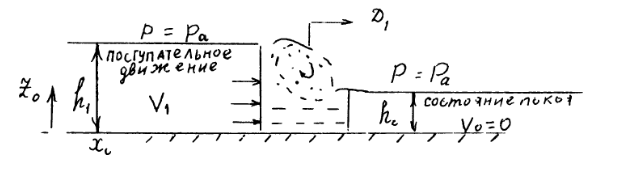
\includegraphics[width=170mm]{pics/1-4-1.png}}
  \caption{Гидравлический прыжок}
  \label{1-4-1}
\end{figure}

Переходная зона -- "ступенька"{} уровня воды на рис. \ref{1-4-1} движется горизонтально слева направо с постоянной скоростью $D_1$ по покоящейся воде глубины $h_0$, вызывая общий подъем уровня воды на величину $\delta h = h_{1}-h_{0}$ и приводя весь слой жидкости в левом полупространстве в состояние поступательного горизонтального движения с постоянной скоростью $V_1$.

Внутри переходной зоны образуются сложные волновые структуры, происходят пространственные турбулентные движения и диссипативные процессы перемешивания жидкости, зачастую с участием пузырьков воздуха. Моделирование здесь осложнено необходимостью учета многих тонких свойств, присущих реальной жидкости. Однако всюду вне переходной зоны течение достаточно простое и справедлив гидростатический закон распределения давления по глубине:
\[
\begin{aligned}
&P_{0} = P_{a} + \rho g (h_{0}-z_{0})\ \ \text{-- справа от переходной зоны},\\
&P_{1} = P_{a} + \rho g (h_{1}-z_{0})\ \ \text{-- слева от переходной зоны}.\\
\end{aligned}
\]
Здесь $P_{a}$ -- атмосферное давление над свободной поверхностью; $\rho$ -- плотность воды; $g$ -- ускорение свободного падения в поле сил тяжести; $z_0$ -- вертикальная координата с началом на горизонтальном дне водоема.

При математическом описании гидравлического прыжка, как сильного разрыва, будем всюду в дальнейшем пренебрегать протяженностью переходной зоны и трением о дно водоема (рис. \ref{1-4-2}, а). Для получения условий на разрыве перейдем к подвижной инерциальной системе координат, связанной с фронтом гидравлического прыжка. Относительно новой (сопутствующей) системы координат обращенное движение жидкости будет установившимся и мы получим ситуацию, показанную на рис. \ref{1-4-2}, б. Здесь
\[
  x_{0} = x-tV_{+},\ \ z_{0}=z,\ \ D_{1} = \left(\frac{dx_0}{dt}\right)_{x=0} = V_{+}
\]
\newpage
\begin{figure}[!htp]
  \center{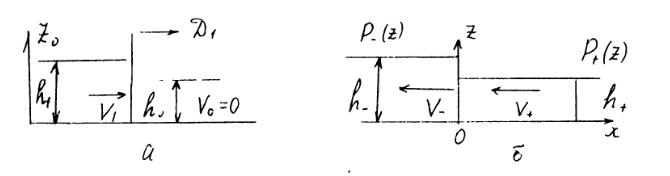
\includegraphics[width=170mm]{pics/1-4-2.png}}
  \caption{}
  \label{1-4-2}
\end{figure}

В системе координат $x,\ z$ на рис. \ref{1-4-2},а состояние жидкости по обе стороны разрыва характеризуется четырьмя параметрами: $h_{\pm}$, $V_{\pm}$. Однако они не могут быть произвольными, а должны удовлетворять соотношениям совместности на разрыве, которые вытекают из общих интегральных законов сохранения для жидких частиц, пересекающих поверхность разрыва $(V_{+}<0,\ V_{-}<0)$:
\addtocounter{equation}{1}
\begin{equation}\label{eq:141}
  V_{-}h_{-} = V_{+}h_{+},
  \tag{1}
\end{equation}
\addtocounter{equation}{1}
\begin{equation}\label{eq:142}
  h_{+}V_{+}^{2} - h_{-}V_{-}^{2} = \frac{g}{2}(h_{-}^{2} - h_{+}^{2})
  \tag{2}
\end{equation}

Вывод этих соотношений достаточно прост и основан на следующих соображениях. Пусть $L$ -- линейный поперечный размер рассматриваемого слоя жидкости в направлении перпендикуляра к плоскости рисунка, например, ширина канала.

За время $\Delta t$ из правого полупространства через неподвижный фронт гидравлического прыжка (справа налево) пройдет масса жидкости $\Delta m_{+} = -V_{+}Lh_{+}\rho \Delta t$. За это же время в левую от фронта прыжка область поступит масса $\Delta m_{-} = -V_{-}Lh_{-}\rho \Delta t$. Поскольку движение установившееся, то для поддержания баланса расхода в слое жидкости необходимо потребовать равенства $\Delta m_{+} = \Delta m_{-} = \Delta m$, которое сводится к соотношению \eqref{eq:141}.

Итак, за время $\Delta t$ жидкий объем массы $\Delta m$ полностью перемещается из правого в левое полупространство, проходя через фронт гидравлического прыжка. При этом изменение количества движения $Q$ данной массы жидкости составит
\[
  \Delta Q = (-\Delta m V_{-}) - (-\Delta m V_{+}) = -\delta m (V_{-} - V_{+}),
\]
а импульс $I$ внешних сил в горизонтальном направлении (см. рис. \ref{1-4-2}, б) за время $\Delta t$ равен
\[
  I = \left[\int\limits_{0}^{h_{+}}P_{+}dz - \int\limits_{0}^{h_{-}}P_{-}dz + P_{a}(h_{1}-h_{+})\right] L \Delta t
\]
С учетом гидростатического распределения для давления $P(z)$
\[
  P_{\pm}(z) = P_{a} + \rho g (h_{\pm} - z),
\]
и после упрощений имеем
\[
  I = \frac{1}{2}\rho g (h_{+}^{2} - h_{-}^{2}) L \Delta t.
\]
Следовательно, уравнение изменения количества движения $\Delta Q = I$ (в проекции на продольное горизонтальное направление) приводит к выражению
\[
  -\Delta m (V_{-} - V_{+}) = \frac{\rho g}{2} (h_{+}^{2} - h_{-}^{2}) L \Delta t,
\]
из которого с учетом выписанных выше представлений для $\Delta m$ получаем соотношение \eqref{eq:142}.

Условия \eqref{eq:141}-\eqref{eq:142} на скачке являются следствием законов сохранения массы и изменения импульса частиц, пересекающих фронт гидравлического прыжка.

Что касается закона сохранения энергии, то он в данном  случае не дает дополнительного соотношения между $V_{\pm}$, $h_{\pm}$ на скачке, поскольку полная энергия частицы не может быть выражена только в терминах $V$ и $h$. Учитывая изменение кинетической энергии, работу сил тяжести и сил давления можно лишь подсчитать рассеивание $\Delta E \geqslant 0$ механической энергии жидкой частицы, пересекающей гидравлический прыжок:
\[
  \Delta m \frac{V_{-}^{2} - V_{+}^{2}}{2} = g\Delta m \frac{h_{+} - h_{-}}{2} + \left( \int\limits_{0}^{h_{-}}P_{-}dz - \int\limits_{0}^{h_{+}}P_{+}dz \right) L \Delta t + \Delta E
\]
Отсюда с учетом \eqref{eq:141}-\eqref{eq:142}, выражения для $P_{\pm}$ и после некоторых преобразований получаем энергическое соотношение на  гидравлическом прыжке в виде
\addtocounter{equation}{1}
\begin{equation}\label{eq:143}
  \frac{\Delta E}{\Delta m} = \frac{1}{4}gh_{-}\left(\frac{h_+}{h_-} - 1\right)^3
  \tag{3}
\end{equation}

Следовательно, в гидравлическом прыжке неизбежны потери механической энергии (на турбулизацию, нагрев, образование коротковолновых шлейфов и т.п.). Причем физически ясное условие $\Delta E \geqslant 0$ исключает существование гидравлических прыжков понижения уровня, поскольку из \eqref{eq:143} получается
\addtocounter{equation}{1}
\begin{equation}\label{eq:144}
  (h_{+} - h_{-})V_{+} \geqslant 0.
  \tag{4}
\end{equation}

Теперь запишем соотношения на скачке для случая распространения гидравлического прыжка в покоящуюся воду. Для этого надо перейти к неподвижной системе координат $x_{0},\ z_{0}$ (см. рис. \ref{1-4-2}):
\addtocounter{equation}{1}
\begin{equation}\label{eq:145}
  \begin{aligned}
  &x_{0} = x - tV_{+},\ \ z_{0} = z,\ \ D_{1} = \left(\frac{dx_0}{dt}\right)_{x=0} = -V_{+}\\
  &V_{0} = V_{+} + D_{1} = 0,\ \ V_{1} = V_{-} + D_{1}\\
  &h_{0} = h_{+},\ \ h_{1} = h_{-}
  \end{aligned}
  \tag{5}
\end{equation}
Поскольку законы механики не меняются при переходе к любой инерциальной системе координат, то можно просто подставить выражения \eqref{eq:145} в условия совместности на скачке \eqref{eq:141}-\eqref{eq:144}. В результате получатся следующие условия на фронте гидравлического прыжка, распространяющегося со скоростью $D_1$ в покоящуюся воду глубины $h_0$ (рис. \ref{1-4-2}, а).
\addtocounter{equation}{1}
\begin{equation}\label{eq:146}
  \begin{aligned}
  & D_{1}h_{0} = (D_{1} - V_{1})h_{1}, \\
  & D_{1}h_{0}V_{1} = \frac{g}{2}(h_{1}^{2} - h_{0}^{2}) \\
  & (h_{1} - h_{0})D_{1} \geqslant 0
  \end{aligned}
  \tag{6}
\end{equation}

Таким образом, при заданной начальной глубине $h_0$ три неизвестных величины $h_1$, $D_1$ и $V_1$ не могут быть произвольными, а должны подчиняться связи \eqref{eq:146} на скачке. Соотношения \eqref{eq:146} мы получили, исходя из общих интегральных законов механики, минуя рассмотрение деталей структуры переходной зоны в гидравлическом прыжке.

Интенсивность разрыва характеризуется относительной высотой
ступени $i_{1} = (h_{1} - h_{0})/h_{0}$. Используя безразмерную величину $i_{1}$, нетрудно из системы \eqref{eq:146} получить следующее представление для $V_1$, $D_1$:
\addtocounter{equation}{1}
\begin{equation}\label{eq:147}
  \begin{aligned}
  & V_{1} = D_{1}\frac{i_{1}}{1+i_{1}}, \\
  & D_{1} = \sqrt{gh_{0}}\left(1 + \frac{3}{2}i_{1} + \frac{1}{2}i_{1}^{2}\right)^{1/2}
  \end{aligned}
  \tag{7}
\end{equation}
Видно, что при любых $i_{1} > 0$ скорость распространения гидравлического прыжка $D_1$ больше, чем предельная величина $C_0$:
\addtocounter{equation}{1}
\begin{equation}\label{eq:148}
  C_{0} = \lim\limits_{i_1 \rightarrow\ 0} D_{1}(i_{1}) = \sqrt{gh_{0}}
  \tag{8}
\end{equation}
Таким образом, скорость распространения бесконечно слабых гидравлических прыжков $(i_1 \rightarrow\ 0)$ на мелкой воде определяется формулой $C_{0} = \sqrt{gh_{0}}$.\\

2. Отражение гидравлического прыжка от вертикальной стенки

Пусть $t_*$ -- момент времени прихода фронта первого гидравлического прыжка к отражающей вертикальной стенке. Картина движения при $t < t_{*}$, $t = t_{*}$ и $t > t_{*}$ показана на рис. \ref{1-4-3}.
\begin{figure}[!htp]
  \center{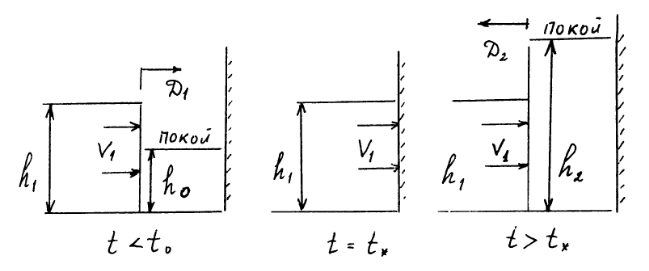
\includegraphics[width=170mm]{pics/1-4-3.png}}
  \caption{Отражение гидравлического прыжка от вертикальной стенки}
  \label{1-4-3}
\end{figure}

Падающий гидравлический прыжок движется с постоянной скоростью $D_1$ по покоящемуся слою воды, ограниченному жесткой вертикальной стенкой. Отраженный гидравлический прыжок движется со скоростью $D_2$ (относительно стенки) навстречу набегающему на стенку слою жидкости с параметрами $V_1$, $h_1$ оставляя за собой состояние покоя $V_2 = 0$, $h_{2} > h_{1}$.

Для получения соотношений на фронте отраженного гидравлического прыжка перейдем, как и раньше, к сопутствующей системе координат, связанной с фронтом отраженного разрыва (рис. \ref{1-4-2}, б), и воспользуемся соотношениями \eqref{eq:141}-\eqref{eq:142}, в которых следует положить
\[
  V_{+} = -V_{1}-D_{2},\ \ V_{-} = -D_{2},\ \ h_{+}=h_{1},\ \ h_{-}=h_{2}.
\]
В результате, после очевидных преобразований, получим искомые соотношения в виде
\addtocounter{equation}{1}
\begin{equation}\label{eq:149}
  \begin{aligned}
  & h_{2}D_{2} = (V_{1}+D_{2})h,\\
  & V_{1}h_{2}D_{2} = \frac{g}{2} \left( h_{2}^{2} - h_{1}^{2} \right)
  \end{aligned}
  \tag{9}
\end{equation}

Соотношения \eqref{eq:146} и \eqref{eq:149} дают полное решение задачи отражения: зная начальную глубину слоя $h_0$ и скорость падающей волны $D_1$, находим из \eqref{eq:146} величины $V_1$, $h_1$, а затем из \eqref{eq:149} находим значения $D_2$, и $h_2$. Если в \eqref{eq:149} вместо $h_2$ ввести интенсивность отраженного разрыва $i_{2} = (h_{2}-h_{1})/h_{1}$, то получим
\[
  \begin{aligned}
  & V_{1} + D_{2} = (1+i_{2})D_{2}\\
  & (1+i_{2})D_{2}V_{1} = gh_{1}i_{2}\left(1+\frac{i_2}{2}\right)
  \end{aligned}
\]
Отсюда
\[
  \begin{aligned}
  & i_{2} = \sqrt{\xi(M_{1})},\\
  & D_{2} = \frac{V_{1}}{\sqrt{\xi(M_{1})}},
  \end{aligned}
\]
где
\addtocounter{equation}{1}
\begin{equation}\label{eq:1410}
  M_{1} = \frac{V_{1}}{\sqrt{gh_1}},\ \ \xi = \left(2-\frac{2}{2+\sqrt{\xi}} \right)M_{1}^{2}
  \tag{10}
\end{equation}
Видно, что уравнение \eqref{eq:1410} имеет единственный корень, который лежит в интервале $\xi \in [M_{1}^{2}, 2M_{1}^{2}]$. Конкретное значение $\xi(M_{1})$ можно найти методом итераций:
\[
  \xi = \lim\limits_{n \rightarrow\ \infty}\xi_{n},\ \ \xi_{n} = \left(2 - \frac{2}{2+\sqrt{\xi_{n-1}}}\right) M_{1}^{2}
\]

\vspace{0.5cm}

\noindent III. \underline{Экспериментальная часть}

1. Описание экспериментальной установки ГАУТ

Установка предназначена для демонстрации и исследования распространения длинных волн в открытом водоеме и их взаимодействия с различными преградами. Название ГАУТ представляет собой аббревиатуру слов "гидравлический аналог ударной трубы". Общая схема устройства ГАУТ показана на рис. \ref{1-4-4}, а. Установка состоит из горизонтального прямоугольного металлического лотка 1 размером 150$\times$75$\times$7 см$^3$, в дно которого вмонтирован микроманометрический датчик давления 2; пружинного механизма 4, обеспечивающего резкий подъем поперечной непроницаемой перегородки 3; электронного блока 7 обработки и регистрации сигналов от датчика давления 2.
\begin{figure}[!htp]
  \center{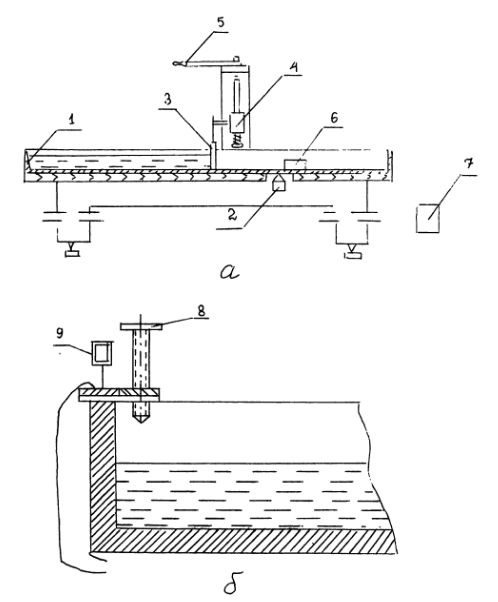
\includegraphics[width=170mm]{pics/1-4-4.png}}
  \caption{}
  \label{1-4-4}
\end{figure}

Установка работает следующим образом. Лоток разделяется на два несообщающихся отсека перегородкой 3 и заполняется водой так, чтобы в отсеках образовывался разный уровень воды. Затем рычагом 5 пружинный механизм 4 приводится в действие, в результате чего перегородка 3 почти мгновенно убирается, имитируя разрушение плотины. Из-за различия первоначальных уровней воды слева и справа от перегородки жидкость приходит в движение: в одну сторону распространяется пологая волна понижения уровня, в другую -- прямолинейный гидравлический прыжок с постоянными параметрами за фронтом (аналог плоской ударной волны в  газодинамической ударной трубе). Датчике измеряет во времени нестационарное давление в жидкости на дне лотка. В областях, где  справедлив гидростатический закон распределения давления по глубине жидкости, показания датчика прямо пропорциональны текущему значению глубины $h$ в данной точке в данный момент времени.

\begin{figure}[!htp]
  \center{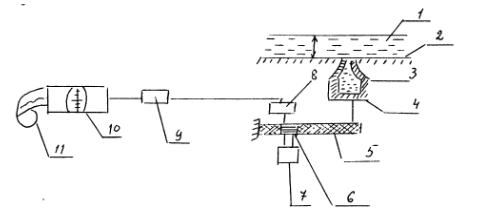
\includegraphics[width=170mm]{pics/1-4-5.png}}
  \caption{Схема измерения глубины слоя воды $h$ в лотке ГАУТ: 1 -- слой воды на горизонтальном дне, 2 -- дно лотка, 3 -- надмембранная полость датчика, 4 -- герметичная мембрана (поршень), 5 -- упругая консоль, 6 -- прозрачный кристалл (фосфид галлия), 7 -- источник света, 8 -- фотодиод, 9 -- усилитель электрического сигнала от фотодиода, 10 -- шлейфовый осциллограф, 11 -- фотобумага}
  \label{1-4-5}
\end{figure}

2. Измерительная система ГАУТ. Тарировка датчика.

Принципиальная схема измерительной системы показана на рис. \ref{1-4-5}.

В зависимости от изменения глубины $h$ слоя воды в лотке изменяется нагружение упругой консоли 5 и оптического кристалла 6, который изменяет свою прозрачность\footnote{Здесь дается упрощенная трактовка принципа работы высокочувствительного прибора, основанного на использовании пьезооптического эффекта.} и соответственно изменяется световой поток на фотодиод 8. В результате образуется переменный (пропорциональный $h$) электрический сигнал, который после усиления в блоке 9 регистрируется осциллографом 10 на фотобумаге 11. Изменение глубины воды в лотке на величину $\Delta h$ вызывает отклонения луча осциллографа на величину $\widetilde{\Delta h} = K\Delta h$. В рабочем диапазоне глубин в лотке $0\leqslant h \leqslant 0.05$м указанная связь близка к линейной: $K = \const (\Delta h)$.

Коэффициент пропорциональности $K$ называется тарировочным коэффициентом. В общем случае он зависит от температуры в помещении и от других факторов, поэтому при подготовке к каждому эксперименту необходимо определять соответствующий тарировочный коэффициент. С этой целью проводится статическая тарировка датчика следующим образом. Над входом в надмембранную полость датчика устанавливаем цилиндрическую трубку диаметра $d$ (рис. \ref{1-4-6}) и регистрируем на осциллограф начальный сигнал $\widetilde{h_0}$, соответствующий некоторому начальному уровню воды в трубке. Затем при помощи дозатора внутрь трубки вводим заданный объем воды $w$, что вызовет подъем уровня воды в трубке на величину $\Delta h_{1} = 4w:(\pi d^{2})$. Соответственно этому луч осциллографа займет новое положение $\widetilde{h_1}$. Затем вводим в трубку следующую порцию воды. Полученный уровень $\Delta h_{2} = 2\Delta h_{1}$ регистрируем на осциллографе и т.д. В результате получаем тарировочную зависимость в виде точек $(\Delta h_{n}, \Delta \widetilde{h_n})$ на плоскости, где по осям отложены: фактический подъем уровня воды над датчиком $\Delta h$ и соответствующее ему отклонение $\Delta \widetilde{h}$ луча осциллографа ($\Delta h_{n} = n\Delta h_{1}$, $\Delta \widetilde{h_n} = \widetilde{h_n} - \widetilde{h_0}$, $n\geqslant 0$). Эту зависимость следует аппроксимировать прямой $\Delta \widetilde{h} = K\Delta h$ (например, по методу наименьших квадратов), в результате чего будет найден тарировочный коэффициент $K$.\\

3. Порядок проведения эксперимента
\begin{enumerate}
  \item Включить измерительную систему.
  \item Провести тарировку датчика.
  \item Заполнить водой правый отсек лотка (с датчиком) до уровня $h = h_{\text{П}}$ ($h_{\text{П}} = 5+10$ мм), левый -- до уровня $h = h_{\text{Л}}$ ($h_{\text{Л}} = 15+30$ мм).
  
  Начальные уровни $h_{\text{Л}}$, $h_{\text{П}}$ определяются электромеханическим измерителем глубины, содержащим винтовой зонд 8 (рис. \ref{1-4-4}, б) со счетчиком оборотов 9 и индикатор скачка проводимости среды между острием винта и корпусом лотка (регистрируем моменты касания зондом поверхности воды и дна лотка).
  
  \item Привести в действие подъемный механизм, наблюдать распространившийся вправо от перегородки гидравлический прыжок, затем отражение этого прыжка от правого борта лотка (скорость "ступеньки"{} составляет 40+50 см/с).
  \item Выключить измерительную систему и обработать осциллограмму рассматриваемого процесса.
\end{enumerate}

Осциллограмма процесса имеет вид, показанный на рис. \ref{1-4-6} ($t$ -- время, на фотобумаге имеется соответствующая временная сетка).
\newpage
\begin{figure}[!htp]
  \center{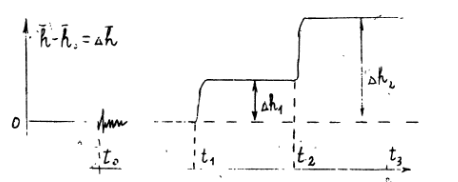
\includegraphics[width=140mm]{pics/1-4-6.png}}
  \caption{}
  \label{1-4-6}
\end{figure}

При $t < t_0$ (до снятия перегородки) имеем базовый сигнал $\widetilde{h_0}$, соответствующий начальное уровню воды $h_{0} = h_{\text{П}}$ в лотке справа. При $t = t_0$ на этот сигнал накладываются вибрации лотка от срабатывания пружинного механизма подъема перегородки. В момент $t = t_1$ гидравлический прыжок достигает точки входа в надмембранную полость датчика; при $t_{1} < t < t_{2}$ сигнал $\Delta \widetilde{h} = \Delta \widetilde{h_1}$ соответствует повышенному уровню воды $\Delta h_{1} = h_{1} - h_{0}$ за первой ступенькой. В момент $t = t_2$ к точке входа в надмембранную полость датчика приходит отраженный от правого борта лотка второй гидравлический прыжок (отраженная ступенька), при $t_{2} < t < t_{3}$ сигнал $\Delta \widetilde{h} = \Delta \widetilde{h_2}$ соответствует повышенному уровню воды $\Delta h_{2} = h_{2} - h_{0}$ между правым бортом лотка и фронтом отраженного гидравлического прыжка, распространяющегося влево. Последующее при $t > t_3$ понижение уровня воды соответствует приходу волны понижения уровня, которая пришла к входу в датчик, отразившись от левого борта лотка. Далее начинается сложный затухающий волновой процесс постепенного выравнивания общего уровня воды в лотке.

Для анализа полученных результатов потребуется знать расстояние $l_1$ от створа "плотины"{} до входа в датчик и расстояние $l_2$ от входа в датчик до отраженной вертикальной стенки. Эти величины, а также $d$, $w$, $h_{\text{Л}}$, $h_{\text{П}}$ измеряются непосредственно, а остальные -- при помощи осциллограммы.\\

\noindent IV. \underline{Обработка и анализ результатов}

\begin{enumerate}
  \item Построить тарировочный график, определить тарировочный коэффициент $K$.
  \item Пользуясь осциллограммой определить величины $\Delta h_{1}$, $\Delta h_{2}$, $\Delta t_{1} = t_{1} - t_{0}$, $\Delta t_{2} = t_{2} - t_{1}$.
  \item Найти экспериментальные значения высоты уровня и скорости перемещения фррнта в падающем и отраженном гидравлическом прыжках $(h_{0} = h_{\text{П}})$:
  \[
    \begin{aligned}
    &h_{1\text{Э}} = h_{0} + \frac{\Delta\widetilde{h_1}}{K},\ \ h_{2\text{Э}} = h_{0} + \frac{\Delta\widetilde{h_2}}{K}\\
    &D_{1\text{Э}} = \frac{l_1}{\Delta t_1},\ \ D_{2\text{Э}} = \frac{l_2}{\Delta t_{2} - l/D_{1\text{Э}}} = \frac{l_2}{\Delta t_{2} - \frac{l_2}{l_1}\Delta t_{1}}
    \end{aligned}
  \]
  Определить также экспериментальные значения интенсивностей падающей и отраженной волн:
  \[
    i_{1\text{Э}} = \frac{h_{1\text{Э}} - h_{0}}{h_0},\ \ i_{2\text{Э}} = \frac{h_{2\text{Э}} - h_{1\text{Э}}}{h_{1\text{Э}}}
  \]
  Составить таблицу экспериментальных результатов:
  \begin{center}
  \begin{tabular}{|c|c|c|c|c|c|c|c|}
  \hline
  $K$ & $h_0$ & $h_{1\text{Э}}$ & $h_{2\text{Э}}$ & $D_{1\text{Э}}$ & $D_{2\text{Э}}$ & $i_{1\text{Э}}$ & $i_{2\text{Э}}$\\
  \hline
  & & & & & & & \\
  \hline
  \end{tabular}
  \end{center}
  
  \item Принимая $i_{1} = i_{1\text{Э}}$ вычислить по соотношениям \eqref{eq:147} на скачке теоретические значения ($C_{0} = \sqrt{gh_0}$, $h_{1} = h_{1\text{Э}}$):
  \addtocounter{equation}{1}
  \begin{equation}\label{eq:1411}
    M_{0} = \frac{D_0}{C_0},\ \ M_{1} = \frac{V_1}{C_1},\ \ C_{1} = \sqrt{gh_1} = C_{0}\sqrt{1 + i_{1}}
    \tag{11}
  \end{equation}
  Определить погрешность $\varepsilon_{1} = (D_{1} - D_{1\text{Э}}) / D_{1} = 1 - \frac{D_{1\text{Э}}}{C_{0}}M_{0}^{-1}$.
  
  \item Найти приближенное решение $\xi_{1} = \xi(M_1)$ уравнения \eqref{eq:1410}, вычислить по соотношениям \eqref{eq:146} теоретические значения интенсивности и скорости отраженного разрыва:
  \[
    i_{2} = \sqrt{\xi_{1}},\ \ D_{2} = \frac{V_1}{\sqrt{\xi_1}}  
  \]
  
  \item Определить погрешности
  \[
    \varepsilon_{2} = \frac{D_{2} - D_{2\text{Э}}}{D_2},\ \  \varepsilon_{3} = \frac{h_{2} - h_{2\text{Э}}}{h_2} = \frac{1 + i_{2} - h_{2\text{Э}}/h_{1\text{Э}}}{1 + i_{2}}
  \]
  Составить итоговую таблицу данных теоретического решения задачи:
  \begin{center}
  \begin{tabular}{|c|c|c|c|c|c|c|c|c|}
  \hline
  $C_0$ & $C_1$ & $D_1$ & $V_1$ & $D_2$ & $h_2$ & $\varepsilon_1$ & $\varepsilon_2$ & $\varepsilon_3$\\
  \hline
  & & & & & & & & \\
  \hline
  \end{tabular}
  \end{center}
\end{enumerate}

\noindent V. \underline{Отражение бора от наклонной стенки}

1. Если линия фронта падающей ударной волны составляет некоторый угол $\alpha > 0$ с отражающей стенкой, то при определенных условиях реализуется так называемое регулярное отражение: возникает отраженная волна с прямолинейным фронтом, начинающимся от места пересечения фронта падающей волны со стенкой. Вполне аналогичное явление наблюдается на мелкой воде. На рис. \ref{1-4-7} показано регулярное отражение бора от вертикальной стенки:
\begin{figure}[!htp]
  \center{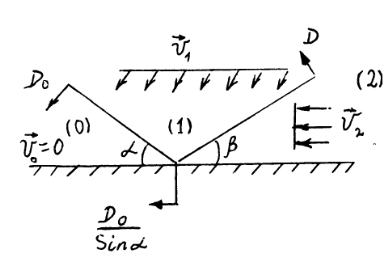
\includegraphics[width=120mm]{pics/1-4-7.png}}
  \caption{}
  \label{1-4-7}
\end{figure}
$\alpha$ и $\beta$ -- углы падения и отражения; $D_0$ и $D_1$ -- скорости падающего и отраженного фронтов, состояния (0) и (1) точно такие же, как при распространении прямолинейного бора в покоящуюся воду; по известному постоянному потоку (1) за падающим бором  распространяется косой бор, оставляя за собой постоянный поток, движущийся вдоль, стенки со скоростью $D_{0}/\sin\alpha$. Последний случай можно исследовать теоретически на основе соотношений динамической совместности на фронтах разрывов в падающей и отраженной волнах.

Если падающая волна является слабой $((h_{1}-h_{0})/h_{0} \ll 1)$, то ее отражение согласуется с законом геометрической акустики, т.е. оба фронта образуют со стенкой одинаковые углы $(h_{2}-h_{0})/h_{0} \approx 2(h_{1}-h_{0})/h_{0}$ независимо от величины угла падения $\alpha$. Однако, если падающая волна сильная и угол ее падения не слишком мал, может создаться положение, когда регулярное отражение невозможно и реализуется сложная ветвящаяся нестационарная система разрывов. Этот случай называется маховским отражением (по имени Э.Маха, впервые описавшего подобные отражения). На рис. \ref{1-4-8} показана тройная конфигурация ударных волн, возникающая при маховском отражении. Теоретическое описание этого явления затруднено. 
\begin{wrapfigure}[6]{l}{0.35\linewidth} 
  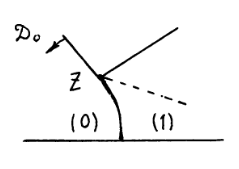
\includegraphics[width=60mm]{pics/1-4-8.png}
  \caption{}
  \label{1-4-8}
\end{wrapfigure}
Отраженный  разрыв ответвляется от падающего в точке $z$, которая движется не параллельно стенке, а удаляется от нее под некоторым углом. Точка разветвления $z$ связана со стенкой перпендикулярным "маховским фронтом"{}, вызывающим течение среды вдоль стенки.

\newpage
2. Лабораторная работа

Провести тарировку датчика глубины. Заполнить лоток водой до глубины $h_{00}$, установить перегородку и отражающую стенку под углом $\alpha$ к перегородке на расстоянии $\approx$ 6 см от датчика глубины; понизить уровень воды в отсеке, содержащем датчик до глубины $h_0$; привести в действие подъемное устройство. Визуально и по полученной осциллограмме определить характер отражения возникающего бора. Описать наблюдаемое явление и объяснить поведение кривой на осциллограмме. В случае регулярного отражения составить таблицу результатов измерений:
\begin{center}
  {\large
  \begin{tabular}{|c|c|c|c|c|c|c|}
  \hline
  $h_{00}$ & $h_0$ & $h_{0}/h_{00}$ & $h_1$ & $h_2$ & $\frac{h_{1}-h_{0}}{h_0}$ & $\frac{h_{2}-h_{0}}{h_0}$\\
  \hline
  & & & & & & \\
  \hline
  \end{tabular}
  }
\end{center}

\noindent VI. \underline{Дифракция бора на ребре излома отраженной стенки}

1. Отражение ударных волн от стенок, содержащих точки и линии разрыва наклона образующей, обладает рядом особенностей. При описании течения среды за фронтом отраженной волны выделяют зоны дифракции и зоны отражения. Зоной дифракции называется область течения "занятая"{} возмущениями, идущими от точек излома отражающей границы.
\begin{wrapfigure}[9]{l}{0.4\linewidth} 
  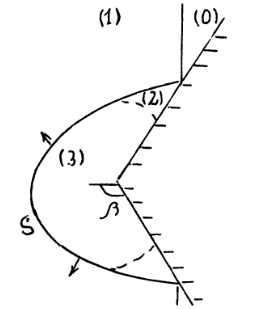
\includegraphics[width=70mm]{pics/1-4-9.png}
  \caption{}
  \label{1-4-9}
\end{wrapfigure}
На рис. \eqref{1-4-9} показана волновая картина взаимодействия плоской ударной волны с клином: область (0) -- невозмущенное состояние среды; (1) -- постоянное течение за падающим разрывом; (2) -- зона отражения; (3) -- зона дифракции; $S$ -- криволинейный участок отраженного фронта, пунктиром показана граница слабых возмущений, идущих от вершины клина по зоне отражения (2).\\

В общем нелинейном случае положение дифрагированного фронта заранее неизвестно, однако в том случае, когда падающая волна является слабой, так что течение в целом описывается линеаризованными уравнениями движения, положение разрывов можно определить независимо от возникающего течения.

Аналогом отражения плоской ударной волны в газе от жесткой границы в виде двугранного угла раствора $2\beta\ (0 < \beta < \pi)$ является отражение прямолинейного бора на мелкой воде от соответствующей вертикальной стенки. При $\pi > \beta > \pi/2$ имеем отражение от стенок клина, при $0 < \beta < \pi/2$ -- от стенок клиновидной воронки, при $\beta = \pi/2$ -- от прямолинейной стенки.

Можно показать, что в областях, куда еще не достигли возмущения от концов щек двугранного угла, течение является автомодельным и в вершине угла параметры среды не зависят от времени.

Если падающая волна слабая $((h_{1}-h_{0})/h_{0} \ll 1)$ то течение описывается волновым уравнением
\[
  \Delta H = \frac{1}{C_{0}^{2}} \pdfrac{^{2}H}{t^{2}},
\]
где
\[
  C_{0} = \sqrt{gh_0},\ \ H = \frac{h - h_{0}}{h_{1} - h_{0}}.
\]
Фронты волн представляют собой отрезки прямых и окружностей, движущихся с постоянной скоростью $C_0$. В этом случае можно  построить в явном виде автомодельное решение задачи отражения от безграничного двугранного угла при всех $0<\beta <\pi$. В частности, в вершине угла получается
\[
  H = \pi / \beta
\]
причем в тех случаях, когда отношение $\pi / \beta$ является целым, это значение распространяется на всю зону дифракции. Например, при $\beta = \pi /4$ в окрестности вершины возникает расширяющаяся с течением времени зона покоя, характеризующаяся глубиной
\[
  h = h_{0} + 4(h_{1} - h_{0}).
\]

2. Лабораторная работа

Провести тарировку датчика глубины. Заполнить лоток водой до глубины $h_{00}$, установить перегородку. Расположить отражающий уголок раствора $2\beta$ симметрично к перегородке так, чтобы датчик глубины находился вблизи вершины уголка. Понизить уровень в отсеке, содержащем модель, до глубины $h_0$. Привести в действие подъёмное устройство. Ориентируясь по непосредственным визуальным наблюдениям и по осциллограмме, охарактеризовать волновую картину вокруг уголка в различные моменты времени. По осциллограмме определить $h_0$, $h_{00}$, а также глубину $h_{*}$ воды в вершине угла на первом этапе отражения (когда эта величина сохраняет постоянное значение) и время $t_0$ прохождения бором расстояния $x_0$ от створа перегородки до вершины уголка. Составить таблицу результатов:
\begin{center}
  \begin{tabular}{|c|c|c|c|c|c|c|c|c|c|c|}
  \hline
  $\pi/\beta$ & $h_{00}$ & $h_{0}$ & $h_*$ & $h_{0}/h_{00}$ & {\Large $\frac{h_{00}-h_{0}}{h_0}$} & $\sqrt{gh_0}$ & $b$ & $\sigma - 1$ & {\Large $\frac{h_{*}-h_{0}}{\frac{1}{2}(h_{00}-h_{0})}$} & {\Large $\frac{h_{*}-h_{0}}{(\sigma - 1)h_{0}}$}\\
  \hline
  & & & & & & & & & &\\
  \hline
  \end{tabular}
\end{center}
где
\[
  \sigma = \frac{4b^2}{1 + \sqrt{1+8b^2}},\ \ b = \frac{x_0}{t_{0}\sqrt{gh_0}}.
\]
\\
ЛИТЕРАТУРА\\
1. Седов Л.И. Механика сплошной среды. Ч.1. М.: Наука, 1973.\\
2. Стокер Дж. Волны на воде. М.: ИЛ, 1959.\\
3. Лайтхилл Дж. Волны в жидкости. М.: Мир, 1981.\\
4. Гилинский М.М., Лебедев М.Г., Якубов И.Р. Моделирование течений газа с ударными волнами. М.: Машиностроение, 1984.

\anonsection{Раздел 2}
\anonsubsection{Задача 1. Волны разгрузки в гибких растяжимых нитях}
\addtocounter{equation}{1}
\begin{equation}\label{eq:1217}
  v_{t_1} = v_{t_2}
  \tag{17}
\end{equation}

\newpage
\anonsubsection{Задача 2. Изучение процесса разгона поршня в стволе пневматической установки}

Целью работы является ознакомление с пневматической установкой и измерительной аппаратурой, теоретическое и экспериментальное определение закона движения поршня, а также определение начальной длины ствола, необходимой для возникновения головной ударной волны.

\noindent I. \underline{Описание явления}

Рассматривается процесс движения поршня в стволе пневмоустановки. Ствол представляет собой полый цилиндр постоянного поперечного сечения, заполненный воздухом. Поршень (снаряд) является металлическим цилиндром массы $M$. Он закрепляется в стартовой позиции с помощью замкового устройства. Размеры снаряда малы по сравнению с длиной ствола. Снаряд разделяет ствол на две части. За поршнем (область I) в начале эксперимента воздух находился под давлением $p_0$ ($p_{0} > p_{\text{атм}}$). Часть ствола, находящаяся перед поршнем (область II) открыта в атмосферу, т.е. давление в ней есть $p_{\text{атм}} = 1 \text{атм}$. В момент $t=0$ поршень освобождается и начинает двигаться в сторону области меньшего давления.
\begin{figure}[!htp]
  \center{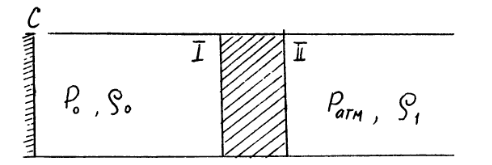
\includegraphics[width=140mm]{pics/2-2-1.png}}
  \caption{}
  \label{2-2-1}
\end{figure}

Введем систему эйлеровых координат. Ось $x$ направим от снаряда в сторону дульного отверстия. Начало координат поместим в точке старта поршня. Волновая картина, сопровождающая разгон поршня, изображена на рис. \ref{2-2-2}. Здесь кривая (0) -- закон движения поршня $(x = X(t))$; прямые (1) -- характеристики, составляющие волну разрежения, распространяющиеся по области I (расходящийся веер); прямые (2) -- характеристики, образующее волну сжатия, распространяющиеся по области II (сходящийся веер); C-C -- стенка, K-K -- конец ствола; кривые (3) -- характеристики волны разрежения, отраженные от стенки. Они искривлены, так как распространяются в движущемся газе. Кривые (4) -- характеристики волны разрежения, появившиеся в результате отражения волны сжатия от свободного конца ствола.

Задача решается в одномерной постановке.
\begin{figure}[!htp]
  \center{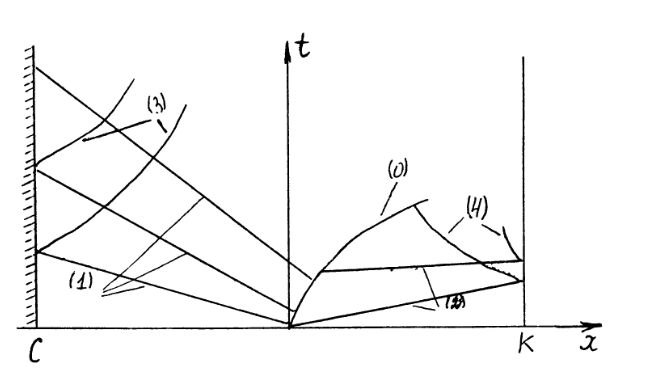
\includegraphics[width=160mm]{pics/2-2-2.png}}
  \caption{}
  \label{2-2-2}
\end{figure}

\noindent II. \underline{Теоретическая часть}

Безволновая теория

Сделаем следующие предположения:\\
1) Пренебрегаем головной волной сжатия и считаем, что во время выстрела на поршень спереди действует только атмосферное давление.\\
2) Пренебрегаем конечностью скорости распространения хвостовой волны разрежения и считаем, что в каждый данный момент времени все параметры воздуха и в тем числе его плотность во всей длине области I постоянна.\\
3) Считаем движение газа изэнтропичным, поэтому давление газа сзади поршня при его движении в стволе будем вычислять по формуле $p = p_0 (\rho / \rho_0)^\gamma $, или
\[
	p = p_0 ( V_0/ (V_0 +S X(t)))^\gamma ,
\]
где $V_0$ -- начальный объем области I; $S$ -- площадь поперечного сечения поршня; $X(t)$ -- координата поршня; $\gamma$ -- показатель адиабаты.

Пусть $M$ -- масса поршня. Запишем при сделанных предположениях уравнение его движения
\[
	M \frac{d^2 X(t)}{ dt^2} = S \left( p_0 \left[\frac{V_0}{V_0 + S X(t)}\right]^{\displaystyle \gamma} - p_{\text{атм}}\right) 
\]
Домножив на $dX/dt$, проинтегрируем его один раз
\addtocounter{equation}{1}
\begin{equation}\label{eq:221}
  \frac{1}{2}M\left(\frac{dX}{dt}\right)^2 = S \left( \frac{p_0V_0}{S (\gamma -1)}\left(1 - \left(\frac{V_0}{V_0 + S X}\right)^{ \displaystyle \gamma -1}\right) - p_{\text{атм}}X\right) 
  \tag{1}
\end{equation}

Сопоставим два члена, разность которых стоит в фигурной скобке. В начальный момент оба члена равны нулю. В конечный момент, когда $X(t) = L$ оба достигают своих наибольших значений. Первый член становится равным
\[
	\frac{p_0V_0}{\gamma -1}\left(1 - \left(\frac{V_0}{V_0 + V_c}\right)^{\displaystyle \gamma -1}\right)
\]
а второй -- $p_{\text{атм}}V_C$, здесь $V_C$ -- объем ствола, $L$ -- длина ствола. Оба растут монотонно. Их максимальные значения при $V_0$ = 650 см$^3$, $V_C$ = 520 см$^3$ имеют отношение
\addtocounter{equation}{1}
\begin{equation}\label{eq:22*}
  p_{\text{атм}} V_{C}\ /\ \left( \frac{p_{0}V_{0}}{\gamma -1}\left(1 - \left(\frac{V_0}{V_0 + V_C}\right)^{\displaystyle \gamma -1} \right)\right) \approx \frac{1}{50} 
  \tag{*}
\end{equation}
Исходя из \eqref{eq:22*}, в правой части \eqref{eq:221} можно оставить только первый член.

Формула \eqref{eq:221} определяет скорость поршня как функцию координаты. Скорость поршня, получаемая из формулы \eqref{eq:221}, будет выше действительной. Это вызвано следующими причинами:
\begin{itemize}
  \item[-] на поршень сзади действует не среднее давление в области
I, а несколько меньшее, так как полна разрежения выравнивает давление не мгновенно;
  \item[-] спереди на поршень действует давление большее, чем $p_{\text{атм}}$, так как перед поршнем распространяется волна сжатия;
  \item[-] есть некоторые потери за счет трения.
\end{itemize}

Волновая теория

При более тонном рассмотрении из предположений предыдущего раздела сохраним только предположение об изэнтропичности течения, т.е. $V/V_0 = \phi(p) = (p/p_0)^{-1/ \gamma}$ в области I и $V/V_1 = \psi(p) = (p/p_{\text{атм}})^{-1/ \gamma} $ для области II. Здесь $V$, $V_0$, $V_1$ -- удельные объемы: $V_0$ -- удельный объем при $t\leqslant 0$ в области I, $V_1$ -- удельный объем при $t\leqslant 0$ в области II, $V$ -- текущее состояние удельного объема, $p$ -- давление в газе. Тогда уравнения движения газа за поршнем (область I) и перед поршнем (область II) запишутся в виде [1]:

\addtocounter{equation}{1}
\begin{equation}\label{eq:222}
  \begin{array}{lr}
  \begin{cases}
    \displaystyle \pdfrac{V}{t} = \displaystyle -\frac{1}{\rho_0} \pdfrac{p}{h} \\
    \displaystyle \pdfrac{\varphi}{t} = \displaystyle \pdfrac{V}{h}
  \end{cases}
  &
  \text{(В области I)}
  \end{array}
  \tag{2}
\end{equation}
\addtocounter{equation}{1}
\begin{equation}\label{eq:223}
  \begin{array}{lr}
  \begin{cases}
    \displaystyle \pdfrac{V}{t} = \displaystyle -\frac{1}{\rho_1} \pdfrac{p}{h} \\
    \displaystyle \pdfrac{\psi}{t} = \displaystyle \pdfrac{V}{h}
  \end{cases}
  &
  \text{(В области II)}
  \end{array}
  \tag{3}
\end{equation}


В формулах \eqref{eq:222}, \eqref{eq:223} введены следующие обозначения: $x(h, t)$ -- координата Эйлера, $h$ -- координата Лагранжа, $h=0$ -- координата поршня, $\rho_{0} = 1/V_{0}$ и $\rho_{1} = 1/V_{1}$ -- начальные плотности в областях I, II соответственно.

Начальные условия для системы \eqref{eq:222}, \eqref{eq:223} таковы:
\addtocounter{equation}{1}
\begin{equation}\label{eq:224}
	\begin{array}{llll}
  		t = 0, & x(h,0) = & \partial x (h, 0)/ \partial t = & 0, \\
  		p(h,0) =  p_0 & (h < 0) ; & p(h,0) =  p_{\text{атм}} &(h > 0).
  \end{array}
  \tag{4}
\end{equation}

Напишем условие при $h=0$, характеризующее движение поршня:
\addtocounter{equation}{1}
\begin{equation}\label{eq:225}
  M \frac{\partial ^2 x (0,t)}{\partial t^2} = \left[p(-0,t) - p(+0,t)\right] S .
  \tag{5}
\end{equation}
Уравнение \eqref{eq:225} определяет закон движения поршня. Длиной поршня пренебрегаем. Масса $M$ располагается между $h = -0$ и $h = +0$.

В силу \eqref{eq:22*} будем считать, что $p(+0,t)\ll p(-0,t)$. Кроме того, выражение для $p(+0)$ справедливо лишь до момента, когда 
головная волна сжатия достигает конца ствола K-K, и отраженная от K-K волна разрежения достигнет поршня. Это время мало. Выражение же для $p(-0)$ справедливо до момента прихода к поршню волны, отраженной от стенки C-C. Это время значительно больше времени прихода отраженной от K-K волны. Тогда \eqref{eq:225} упростится
\addtocounter{equation}{1}
\begin{equation}\label{eq:226}
  M \frac{\partial ^2 x (0,t)}{\partial t^2} = S p(-0,t)   .
  \tag{6}
\end{equation}
На рис. \ref{2-2-2} показано, что в момент $t=0$ по газу, расположенному слева от поршня начнет распространяться простая волна разрежения. Волна разрежения характеризуется постоянством инварианта Римана [2]:
\[
	s = v + \int\limits^p_{p_0} \sqrt{ - \phi '(\eta) / \rho_0} d\eta = \const, \quad v = \pdfrac{x}{t}. 
\]
Из начального условия следует, что
\addtocounter{equation}{1}
\begin{equation}\label{eq:227}
    v + \int\limits^p_{p_0} \sqrt{ - \phi '(\eta) / \rho_0} d\eta = 0 \quad \text{при} \quad h < 0 .
  \tag{7}
\end{equation}
Решая \eqref{eq:227} относительно $p$, получим выражение $p(-0,t)$ как функцию $v(0,t)$:
\addtocounter{equation}{1}
\begin{equation}\label{eq:228}
	p(-0,t) = p_0 \left[ \frac{1-\gamma}{2 a_1} v(0,t) +1 \right]^{\frac{\displaystyle 2 \gamma}{\displaystyle \gamma - 1}}
  \tag{8}
\end{equation}
Из \eqref{eq:226} и \eqref{eq:228}
\addtocounter{equation}{1}
\begin{equation}\label{eq:229}
	M \frac{d ^2 X(t)}{d t^2} = S p_{0} \left[\frac{1-\gamma}{2 a_1} \frac{d X(t)}{dt} +1 \right]^{\frac{\displaystyle 2 \gamma}{\displaystyle \gamma - 1}}
  \tag{9}
\end{equation}
где $X(t) = x(0,t);$ $ v(t,0) = dX(t)/dt$; $a_1 = \sqrt{\gamma p_0/ \rho_0}$.

Начальные условия для уравнения \eqref{eq:229} имеют вид :
\addtocounter{equation}{1}
\begin{equation}\label{eq:2210}
	t = 0, \quad X = dX / dt = 0 .
  \tag{10}
\end{equation}
Уравнения \eqref{eq:229} с начальными условиями \eqref{eq:2210} легко интегрируются:
\[
	\frac{dX}{dt} = \frac{2 a_1}{\gamma - 1} \left[ 1 - \left( \frac{Sp_0}{M} \frac{\gamma + 1}{2 a_1} t +1 \right) ^{-\frac{\displaystyle \gamma - 1}{\displaystyle \gamma +1 }} \right], 
\]

\[ 
	X = \frac{2a_1}{\gamma - 1}\left[t - \frac{Ma_1}{S p_0}\left( \frac{Sp_0}{M} \frac{\gamma +1}{2 a_1}t +1 \right)^{\displaystyle \frac{2}{ \displaystyle \gamma +1}} + \frac{Ma_1}{Sp_0} \right].
\]
Полученное решение справедливо до момента прихода отраженной от стенки С-С волны к поршню.

Определение наименьшей длины трубы, при которой возможно возникновение ударной волны

Рассмотрим вопрос о возникновении ударной волны в области II.

Как видим на рис. \ref{2-2-2}, веер характеристик положительного  наклона в области II является сходящимся (волны сжатия). Уравнение этих характеристик имеет вид
\begin{center}
		\begin{tabular}{c c c}
			$ \displaystyle \frac{dh}{dt} = \displaystyle \frac{1}{\sqrt{-\rho_1 \psi ' (p)}} $ & $\text{или}$ & 
			$ \left\{
    			\begin{array}{lcl}  
     	 			h &=& \displaystyle \frac{(t-\tau)}{\sqrt{-\rho_1 \psi '(p(\tau))}} , \\
     	 			p &=& p(\tau)
    			\end{array}
  			\right.$ \\
		\end{tabular} 
\end{center}
Точки $\tau$ лежат на прямой $h = 0$.

Ударная волна возникает там, где впервые (т.е. при наименьшем $h$) пересекутся эти характеристики. Очевидно, что первое пересечение характеристик -- это пересечение двух бесконечно близких. Найдем это условие.

Запишем уравнения близких характеристик
\[
	h\sqrt{- \rho_1 \psi' (p(\tau)) } = t- \tau;
\]
\[
	h\sqrt{- \rho_1 \psi' (p(\tau + d\tau)) } = t- (\tau + d\tau) .
\]
Определим при каком наименьшем $h=h^*$ они пересекутся. Решив задачу об их пересечении, устремим $d\tau$ к 0 и обнаружим, что значение $h^*$ определится из уравнения
\[
	h^* = - \frac{1}{\left(\sqrt{- \rho_1 \psi' (p(\tau))} \right) _{\tau}' }
\]
Волна сжатия, распространяющаяся в области II, характеризуется постоянством инварианта Римана
\[
	r \equiv v - \int\limits^{p}_{p_{\text{атм}}} \sqrt{- \psi'(\eta)/\rho_1}\ d\eta,
\]
или
\[
	v - \int\limits^{p}_{p_{\text{атм}}} \sqrt{- \psi'(\eta)/\rho_1}\ d\eta\ =\ 0 \quad \text{при} \quad h > 0.
\]
Выражая из последнего равенства $p$ как функцию $v$, получим
\[
	p = p_{\text{атм}} \left( \frac{\gamma - 1}{2 a_2}v + 1 \right)^{\displaystyle \frac{2\gamma}{\gamma - 1}} .
\]
Учитывая выражения для функций $\psi$ и $p$, получим
\[
	h^* = \frac{2}{\gamma + 1} \frac{a_2^2}{d^2x/dt^2} \left( \frac{\gamma - 1}{2 a_2} \frac{dx}{dt} +1  \right)^{\displaystyle \frac{2\gamma}{\gamma - 1}},
\]
откуда видим, что с ростом $\tau$ значение $h^*$ увеличивается, следовательно, ударная волна возникает на пересечении головной характеристики с бесконечно близкой. Устремляя $\tau$ к нулю, найдем нужное значение
\[
	h^* = \frac{2}{\gamma + 1} \frac{a_2^2 M}{\ddot{x}(0)}
\]
(при $\tau=0$ лагранжева и эйлерова координаты совпадают), где $\ddot{x}(0)$ определяется из уравнения
\[
	\ddot{x}(0) = S (p_0 - p_{\text{атм}})
\]
Тогда
\[
	h^* = \frac{2}{\gamma + 1} \frac{a_2^2 M}{S (p_0 - p_{\text{атм}}) }
\]

\noindent III. \underline{Экспериментальная часть}

Наша задача состоит в экспериментальном определении скорости движения поршня.

1. Описание установки

Устройство установки показано на рис. \ref{2-2-3}. Сжатый воздух,  имеющий давление 200 атм, поступает из магистрального трубопровода 22 через вентиль 15 в редуктор 14. Редуктором 14 снижают давление сжатого воздуха до величины потребной для эксперимента. Сжатый воздух, прошедший через редуктор 14 накапливается во вспомогательном баллоне 13. Перед выстрелом, предварительно закрепив поршень 2 спусковым устройством 3, сжатый воздух из баллона 13 подают через вентиль 17 в баллон 1 установки до заданного для эксперимента давления $p_0$. Величина давления в баллоне 1 контролируется по образцовому манометру 21. В случае, если давление в баллоне будет выше заданного, то избыток давления стравливает через вентиль 17 в атмосферу. Когда давление в баллоне 1 достигает заданного $p_0$, закрывают вентиль 17, включают электромотор шлейфового осциллографа 6 и тумблер 10. Затем нажатием на кнопку 12 производится выстрел. При нажатии на кнопку 12 срабатывает реле 7 запуска съемки осциллографа H-115. После прохождения 5-10 см пленки осциллограф замыкает электроцепь клапана ЭК-48. При срабатывании ЭК-48 воздух из баллона 13 поступает в цилиндр спускового устройства 3, в результате поршень 2 освобождается и под действием давления воздуха, находящегося в баллоне 7 выстреливается из ствола.
\begin{figure}[!htp]
  \center{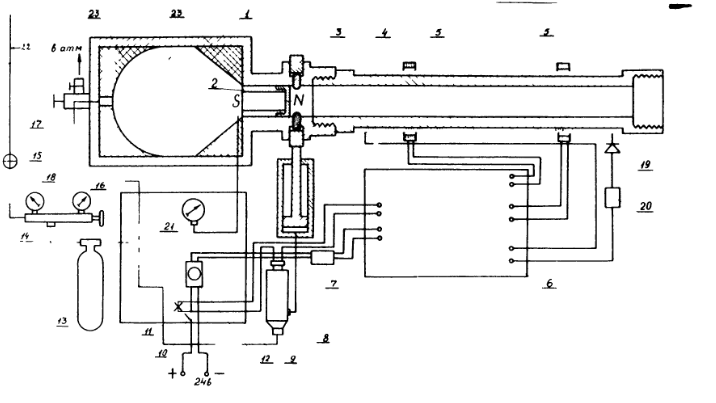
\includegraphics[width=170mm]{pics/2-2-3.png}}
  \caption{}
  \label{2-2-3}
\end{figure}

На стволе 4, изготовленном из диамагнитного материала, имеется специальная обмотка. При движении намагниченного поршня 2 в обмотке ствола индуцируется некоторая электродвижущая сила. Число витков на 1 см длины обмотки неодинаково, а возрастает в арифметической прогрессии по длине ствола. Магнитный поток через всю обмотку есть сумма магнитных потоков через плоскость каждого витка. При этом, если по обе стороны магнита число витков на единицу длины одинаково, то при движении такого магнита полный поток через контур не изменяется и ЭДС не возникает. Если же количество витков на единицу длины катушки возрастает, то магнитный поток, создаваемый одним из полюсов магнита, отличается по абсолютной величине и противоположен по знаку магнитному потоку от другого полюса. При этом оба магнитных потока возрастают по величине с ростом плотности обмотки, следовательно, их сумма тоже возрастает, поскольку она отлична от нуля. Таким образом в обмотке возникает ЭДС индукции, пропорциональная скорости изменения магнитного потока, которая в свою очередь определяется скоростью движения магнита и изменением количества витков на единицу длины вдоль катушки. Так как у нас изменение количества витков линейно, то ЭДС индукции пропорциональна скорости.

Покажем то же самое аналитически. Пусть $x(t)$ -- координата заднего (южного) полюса магнита; $x(t) + l$ -- координата переднего (северного) полюса магнита (рис. \ref{2-2-4}). Здесь $m$ и $-m$ -- магнитные массы северного и южного полюсов магнита (магнитная масса вводится по аналогий с законом Кулона для электрических зарядов); $R$ -- радиус обмотки ствола.
\begin{figure}[!htp]
  \center{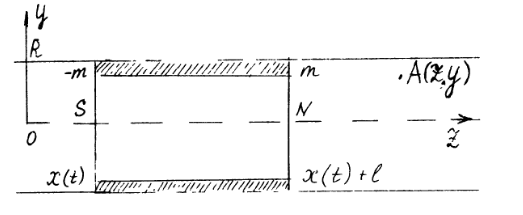
\includegraphics[width=150mm]{pics/2-2-4.png}}
  \caption{}
  \label{2-2-4}
\end{figure}
Рассмотрим один моток ствола, имеющий координату $z$. Проекция вектора напряженности магнитного поля на ось $z$ в  некоторой точке $A(x,y)$:
\[
	H_z(z,y) = \frac{m}{(z-x-l)^2 + y^2} \frac{z-x-l}{\sqrt{(z-x-l)^2 + y^2}} - \frac{m}{(z-x)^2 + y^2} \frac{z-x}{\sqrt{(z-x)^2 + y^2}} .
\]
Найдем магнитный поток через рассматриваемый виток:
\begin{equation}
	\begin{array}{l}
		\Phi(z,t) = \displaystyle \int H_z(z,y) ds = 2 \pi m \displaystyle \int\limits_0^R \left\{ \displaystyle \frac{z-x-l}{\left[ (z - x - l)^2 +y^2 \right]^{3/2}} - \frac{z - x}{\left[ (z - x)^2 + y^2 \right]^{3/2}} \right\} \cdot \\
		\cdot y dy = 2 \pi m \left[ \displaystyle \frac{z-x}{\sqrt{(z-x)^2 + R^2}} - \frac{z - x - l}{\sqrt{(z - x - l)^2 + R^2}} + sign(z - x - l) - \right. \\ 
		- sign(z - x) \Bigg] .
	\end{array}
	\notag
\end{equation} 
ЭДС индукции в витке вычислится по формуле
\begin{equation}
	\begin{array}{l}
	E(z,t) = \displaystyle \frac{\partial \Phi}{\partial t} = - 2 \pi m \displaystyle \frac{dx}{dt} \left[ \frac{1}{\sqrt{(z-x)^2 + R^2}} \frac{1}{\sqrt{(z- x - l)^2 + R^2}} + \right. \\ \left. \displaystyle + \frac{(z - x - l)^2}{\left[ (z - x - l)^2 + R^2 \right]^{3/2}} - \frac{(z - x)^2}{\left[ (z - x)^2 + R^2 \right]^{3/2}} \right] .
	\end{array}
	\notag
\end{equation}

Пусть число витков на 1 см длины обмотки определяется формулой $n(z) = Nz$, где $N$ -- постоянное число. Тогда полная ЭДС индукции во всей катушке длиной $h$ запишется в виде
\begin{equation}
	\begin{array}{l}
	E_n(t) = \displaystyle \int\limits_0^h n(z) E(z,t) dz =  2 \pi m N R^2 \frac{dx}{dt} \left\{ \frac{1}{\sqrt{x^2 + R^2}} + \frac{1}{\sqrt{(x + l)^2 + R^2}} - \right. \\ 
	\left. \displaystyle -\frac{1}{\sqrt{(h - x)^2 + R^2}} - \frac{1}{\sqrt{(h - x - l)^2 + R^2}}  + \frac{x}{R^2}\left[ \frac{(h - x)}{\sqrt{ (h-x)^2 + R^2 }} - \right. \right. \\ 
	\left. \left. \displaystyle -  \frac{(h - x - l)}{\sqrt{ (h - x - l)^2 + R^2 }} + \frac{x}{\sqrt{x^2 + R^2}} - \frac{x + l}{\sqrt{(x + l)^2 + R^2}} \right] \right\} .
	\end{array}
	\notag
\end{equation}

Предположим, что поршень находится внутри катушки на достаточном удалении от ее концов. Тогда $R/x \ll 1$ и $R/(h-x) \ll 1$. Разлагая правую часть формулы для $E_{n}(t)$ по этим малым параметрам, имеем
\addtocounter{equation}{1}
\begin{equation}\label{eq:2211}
	E_n(t) = 4 \pi m l N \frac{dx}{dt} .
  \tag{11}
\end{equation}
Таким образом, ЭДС индукции пропорциональна скорости движения поршня.

Сигнал с обмотки ствола через дополнительное сопротивление 20 подается на шлейфовый осциллограф 6, где и записывается. Тарировка установки производится при помощи двух коротких вспомогательных катушек 5. Эти катушки фиксируют на основной осциллограмме момент пролета поршня мимо них.

Пусть координаты вспомогательных катушек будут $x_1$ и $x_2$, а моменты пролета поршня через эти точки -- $t_1$ и $t_2$. Если пренебречь индуктивностью обмотки, то, как следует из формулы \eqref{eq:2211}, скорость движения поршня можно записать о виде
\addtocounter{equation}{1}
\begin{equation}\label{eq:2212}
	\dot{x}(t) = \frac{dx (t)}{dt} = ky(t),
  \tag{12}
\end{equation}
где $y(t)$ -- амплитуда отклонения шлейфа; $k$ -- тарировочный коэффициент, постоянный для данного выстрела.

Интегрируя \eqref{eq:2212} от $t_1$ до $t_2$, имеем
\addtocounter{equation}{1}
\begin{equation}\label{eq:2213}
	k = \frac{x_2 - x_1}{ \int\limits^{t_2}_{t_1} y(t)dt} ,
  \tag{13}
\end{equation}
где $\int\limits^{t_2}_{t_1} y(t)dt$ вычисляется численным интегрированием по осциллограмме, а $x_2 - x_1$ замеряется на установке.

Из формул \eqref{eq:2212}, \eqref{eq:2213} для скорости поршня получим формулу 
\addtocounter{equation}{1}
\begin{equation}\label{eq:2214}
	\dot{x}(t) = \frac{x_2 - x_1}{ \int\limits^{t_2}_{t_1} y(t)dt} y(t) \equiv k y(t) 
  \tag{14}
\end{equation}
Интегрируя \eqref{eq:2214} от $t_1$ до $t$, получим
\addtocounter{equation}{1}
\begin{equation}\label{eq:2215}
	x(t) = x_1 + \frac{x_2 - x_1}{ \int\limits^{t_2}_{t_1} y(t)dt}  \int\limits^{t}_{t_1} y(t)dt = x_1 + k  \int\limits^{t}_{t_1} y(t)dt.
  \tag{15}
\end{equation}
Формулы \eqref{eq:2214} и \eqref{eq:2215} позволяют определить скорость поршня как функцию его координаты $\dot{x} = f(t) $.\\

2. Порядок выполнения работы\\
1) Произвести необходимые замеры параметров установки, взвесить поршень, проверить его намагниченность.\\
2) Привести в готовность осциллограф.\\
3) Зарядить пушку. Зарядку пушки произвести при отсутствии давления в системе питания установки. Всем покинуть бокс МАУ—20. Находиться в боксе МАУ-20 после подачи давления в систему питания \underline{строго воспрещается}!\\
4) Подать воздух в баллон 1 до давления $p_0$ - 21 атм.\\
5) Произвести выстрел.\\
6) Проявить на свету осциллограмму.\\
7) С осциллографа снять значения $y(t)$ в достаточном числе точек, определить значения интегралов для различных времен $t$: $\int_{t_1}^{t} y(t)dt$, а также интеграл $\int_{t_1}^{t_2} y(t)dt$.\\

\noindent IV. \underline{Обработка и анализ результатов}

В протокол задачи включается:\\
1) Расчет тарировочного коэффициента.\\
2) График $\dot{x} = f(x)$ полученный из эксперимента.\\
3) Графики $\dot{x} = f(x)$, полученные по теоретическим формулам.\\
4) Наименьшее значение $h=h^*$, когда возникает ударная волна.\\

При сравнении результатов эксперимента и теорий необходимо помнить, что экспериментальные формулы дают скорость поршня лишь для $x$: $x_{1} \leqslant x \leqslant x_{2}$, а теоретические зависимости дают скорость по всей длине ствола.

\begin{center}
ЛИТЕРАТУРА
\end{center}
1. Созоненко Ю.А. Движение поршня под действием давления газа // ПММ. 1963. Т.27. Вып.3. С.535-540.\\
2. Уизем Дж. Линейные и нелинейные волны. М.: Мир. 1977.

\newpage
\anonsubsection{Задача 3. Нелинейные волны сжатия (растяжения) сдвига в тонкостенной цилиндрической трубе}

Целью работы является ознакомление с теорией нелинейноупругих волн сжатия (растяжения)-сдвига и экспериментальное изучение волн сжатия (растяжения)-сдвига, вызванных продольным ударом по торцу предварительно закрученного тонкостенного цилиндрического образца.\\

\npart{I}{Описание явления}

Нелинейные волны в твердых деформируемых телах обычно возникают при интенсивных динамических воздействиях, когда связь между напряжениями и деформациями становится нелинейной. Довольно хорошо изучены продольные нелинейные волны (нелинейноупругие, упругопластические, вязко-упругопластические и др.), распространяющиеся в длинных тонких стержнях [1]. Для их теоретического и экспериментального исследований достаточно изучения возмущений только одной, продольной компоненты физических величин: компоненты вектора скорости частиц, тензоров деформации и напряжений и др. Гораздо сложнее обстоит дело в случае, когда нелинейная волна возмущает одновременно несколько компонент физических величин. Математическое описание таких многокомпонентных волн приводит к краевым задачам для квазилинейных гиперболических систем уравнений выше третьего порядка.

Чисто технические и измерительные трудности имеют экспериментальные исследования. Однако основная проблема здесь состоит в интерпретации опытных данных. Прохождение многокомпонентной волны через какую-либо физическую точку среды вызывает в ней процесс нагружения и деформации [4]. В эксперименте возможна прямая регистрация только кинематических величин. Поэтому доступной для опытного определения оказывается только часть процесса, именно процесс деформации. Задача определения полного образа процесса -- одновременная регистрация процессов деформации и нагружения -- остается пока не решенной. В настоящее время существует возможность применения обратного метода: предполагается, что в эксперименте проходит некоторый процесс, в котором соотношения между напряжениями и деформациями известны, решается теоретически в этих предположениях соответствующая эксперименту краевая задача и сравнивается процесс деформации, полученный опытным и теоретическим путем. При их совпадении (с заданной точностью в заданной норме) можно предположить, что и весь процесс проходит так, как это было предположено. О единственности решения при таком подходе пока ничего не известно. Число решенных теоретически задач тоже очень велико. Отметим, что впервые проблема многокомпонентных волн была поставлена и получила определенное теоретическое решение в работах Х.А.Рахматулина [2,3].

\npart{II}{Теоретическая часть}

Теория нелинейноупругих простых волн (волн Римана)

Рассмотрим распространение по полубесконечной тонкостенной круглой трубе одномерных плоских возмущений сжатия (или растяжения)-сдвига.

\begin{wrapfigure}[9]{l}{0.5\linewidth} 
  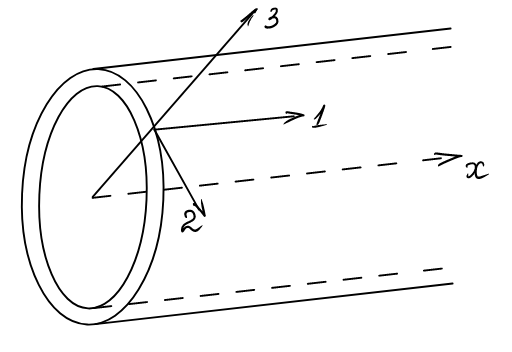
\includegraphics[width=80mm]{pics/2-3-1.png}
  \caption{}
  \label{2-3-1}
\end{wrapfigure}
В покоящейся недеформированной трубе введем  следующую ортогональную лагранжеву систему координат (рис. \ref{2-3-1}). От заданной точки на срединной окружности торца отсчитываются в направлении 1 оси цилиндра координата $x_1$ в направлении 2 касательной к срединной окружности -- $x_2$, в направлении радиуса (по толще стенки) -- $x_3$.

Обозначим $\overrightarrow{w} (w_{1}, w_{2}, w_{3})$ -- вектор перемещения частиц, $\overrightarrow{V} (v_{1}, v_{2}, v_{3})$ -- вектор скорости частиц, $\sigma_{ij}$ -- компоненты тензора напряжений Пиолы - Кирхгоффа, $\varepsilon_{ij}$ -- компоненты тензора малых деформаций.

Пусть начальное состояние трубы однородно и задано следующим образом:
\addtocounter{equation}{1}
\begin{equation}\label{eq:231}
	\begin{array}{l}
		x_1 \geqslant 0, \quad  \overrightarrow{V} = 0, \quad \sigma_{11} = \sigma_{11}^0 = const, \quad \sigma_{12} = \sigma_{12}^0 = const, \\ \sigma_{22} = \sigma_{13} = \sigma_{23} = \sigma_{33} = 0.
	
	\end{array}
  \tag{1}
\end{equation}

Зададим граничные условия. В момент $t=0$ к поверхности $x_{1}=0$ торца трубы прикладываются динамические нагрузки, имеющие не больше двух ненулевых составляющих: продольную (вдоль оси $x_1$) и крутящую (но касательной к срединной окружности). Эти нагрузки однородные: они не зависят от $x_2$, $x_3$, $t$.

Так как толщина стенки трубы мала (по сравнению с радиусом) и боковые поверхности свободны от внешних нагрузок, можно считать, что труба находится в обобщенном плоском напряженном состоянии, т.е. все неизвестные зависят только от $x_1$, $x_2$, $t$ и, кроме того,
\addtocounter{equation}{1}
	\begin{equation}\label{eq:232}
		 \sigma_{13} = \sigma_{23} = \sigma_{33} = 0, \quad \forall x_1, x_2, t
  	\tag{2}
	\end{equation}

Ввиду того, что краевые (начальные и граничные) условия зависят только от $x_1$, предположим, что и само решение есть функция только $x_1$, $t$, т.е.
\addtocounter{equation}{1}
	\begin{equation}\label{eq:233}
		\overrightarrow{V} = \overrightarrow{V}(x,t), \quad \varepsilon_{ij} = \varepsilon_{ij}(x,t), \quad \sigma_{ij} = \sigma_{ij}(x,t),	 
  	\tag{3}
	\end{equation}
где для краткости обозначено 
\[ x = x_1 \]

Для упрощения решения пренебрежем радиальной инерцией, тогда $\sigma_{22} = 0$ для любых $x, t$.

В этих предположениях уравнения движения имеют вид 
\addtocounter{equation}{1}
\begin{equation}\label{eq:234}
		\rho\frac{\partial v_1}{\partial t} = \frac{\partial \sigma_{11}}{\partial x} , \quad \rho\frac{\partial v_2}{\partial t} = \frac{\partial \sigma_{12}}{\partial x}, \quad	\rho\frac{\partial v}{\partial t} = 0, 
  	\tag{4}
\end{equation}
где $\rho$ - плотность недеформированного материала трубы.

Когда начальные и граничные нагрузки не столь велики, то деформации, вызванные ими, малы, т.е. верны формулы Коши
\[
	\varepsilon_{ij} = \frac{1}{2}\left( \frac{\partial w_i}{\partial x_j} + \frac{\partial w_j}{\partial x_i} \right)
\]
откуда следует, что 
\[
	\varepsilon_{11} = \frac{\partial w_1}{\partial x}, \quad \gamma_{12} = 2 \varepsilon_{12} = \frac{\partial w_2}{\partial x},
\]
где $\gamma_{12}$ - полный сдвиг.

В областях непрерывного движения равны вторые смешанные производные по $x$ и $t$ от компонент перемещений. Следовательно,
\addtocounter{equation}{1}
\begin{equation}\label{eq:235}
		\frac{\partial \varepsilon_{11}}{\partial t} = \frac{\partial v{1}}{\partial x} , \quad \frac{\partial \gamma_{12}}{\partial t} = \frac{\partial v_{2}}{\partial x}. 
  	\tag{5}
\end{equation}

Систему \eqref{eq:234}, \eqref{eq:234} замыкают определяющие уравнения.

Моделируем материал трубы нелинейноупругой среды, для которой упругий потенциал $W$ задается соотношением
\[
	dW = \sigma_{\text{ср}}d\varepsilon_{\text{ср}} + \sigma_{u}d\varepsilon_u
\]
где $\sigma_{\text{ср}},\ \varepsilon_{\text{ср}}$ -- средние напряжение и деформация; $\sigma_{u},\ \varepsilon_{u}$ -- интенсивности напряжений и деформаций, определяемые по формулам
\addtocounter{equation}{1}
\begin{equation}\label{eq:236}
		\begin{array}{lll}
			\sigma_{\text{ср}} &=& \displaystyle \frac{1}{3} \sigma_{ii},\\
			\sigma_u &=& \left(\displaystyle \frac{3}{2} (\sigma_{ij} - \sigma_{\text{ср}}\delta_{ij})(\sigma_{ij} - \sigma_{\text{ср}}\delta_{ij}) \right)^{1/2},\\
			\varepsilon_{} &=& \displaystyle \frac{1}{3} \varepsilon_{ii},\\
			\varepsilon_u &=& \left(\displaystyle  \frac{2}{3} (\varepsilon_{ij} - \varepsilon_{\text{ср}}\delta_{ij})(\varepsilon_{ij} - \varepsilon_{\text{ср}}\delta_{ij}) \right)^{1/2}.
		\end{array}
  	\tag{6}
\end{equation}
Здесь предполагается суммирование по повторяющимся индексам, $\delta_ij$ символ Кронекера.

Функции $\sigma_{u} = \Phi(\varepsilon_{u})$ и $\sigma_{\text{ср}} = f(\varepsilon_{\text{ср}})$ являются универсальными для данного материала и находятся из экспериментов на однокомпонентное нагружение, -- динамическое или статическое.

Теперь используя соотношение
\[ 
  \sigma_{ij} = \pdfrac{W}{\varepsilon_{ij}},
\]
получим выражения компонент тензора напряжений от компонент тензора деформаций
\addtocounter{equation}{1}
\begin{equation}\label{eq:237}
		\begin{array}{l}
			\sigma_{ij} - \sigma_{\text{ср}}\delta_{ij} =\displaystyle  \frac{2}{3} \frac{\Phi(\varepsilon_u)}{\varepsilon_u} (\varepsilon_{ij} - \varepsilon_{\text{ср}}\delta_{ij}), \\
			\sigma_{\text{ср}} = f(\varepsilon_{\text{ср}}).
		\end{array}
  	\tag{7}
\end{equation}
	
Отметим, что эти соотношения совпадают с соотношениями теории малых упругопластических деформаций. Следовательно, данная модель нелинейноупругого тела описывает также поведение упругопластического материала в активном процессе.

Для упрощения математической задачи предположим, что материал трубы объемно-несжимаемый, т.е.
\[ \varepsilon_{\text{ср}} = 0 \]
Тогда из соотношений \eqref{eq:232} и \eqref{eq:237} следует, что
\addtocounter{equation}{1}
\begin{equation}\label{eq:238}
	 \varepsilon_{13} = \varepsilon_{23} = 0, \quad \varepsilon_{22} = \varepsilon_{33} = - \frac{1}{2}\varepsilon_{11}. 
	\tag{8}
\end{equation} 
Заменим $\sigma_{11}$, $\sigma_{12}$ определенные уравнениями \eqref{eq:237}, в уравнениях \eqref{eq:234} и выражениями, используя формулы \eqref{eq:238}.
\addtocounter{equation}{1}
	\begin{equation}\label{eq:239}
		\begin{array}{l}
			\displaystyle \frac{\partial \varepsilon}{\partial t} = \displaystyle \frac{\partial u}{\partial x}, \quad \displaystyle \frac{\partial \gamma}{\partial t} = \displaystyle \frac{\partial v}{\partial x}, \\
			\displaystyle \frac{\partial u}{\partial t} = \displaystyle \frac{1}{\rho} \frac{\partial (\varepsilon \phi(s))}{\partial x}, \quad \displaystyle \frac{\partial v}{\partial t} = \displaystyle \frac{1}{3 \rho} \frac{\partial (\gamma \phi(s))}{\partial x},
		\end{array}
  	\tag{9}
	\end{equation}
где для краткости обозначено 
\[ 
	\begin{array}{l}
		u = v_1, \quad v = v_2, \quad \varepsilon = \varepsilon_{11}, \quad \gamma = \gamma_{12}, \\
		s = \varepsilon_u = (\varepsilon^2 + \gamma^{2/3})^{1/2}, \quad \phi(s) = \Phi(s)/s.
	\end{array}
\]

Система уравнений \eqref{eq:239} квазилинейная. Найдем ее характеристики [5]. С этой целью, введя вектор-столбец неизвестных функций
\[
	\overrightarrow{u} = \left[
		\begin{array}{l}
		\varepsilon\\ \gamma \\ u \\ v
		\end{array}
	    \right]
\]
Запишем ее в матричной форме
\addtocounter{equation}{1}
\begin{equation}\label{eq:2310}
		\begin{array}{l}
			\displaystyle \frac{\partial \overrightarrow{u}}{\partial t} = A(\overrightarrow{u})\displaystyle \frac{\partial \overrightarrow{u}}{\partial x},  \\
			A(\overrightarrow{u}) = \left[
			\begin{array}{cc}
				\overrightarrow{0} & I \\ A_1 & \overrightarrow{0}
			\end{array}
			\right],
		\end{array}
  	\tag{10}
\end{equation} 
где $I$, $\overrightarrow{0}$ -- единичная и нулевая матрицы второго порядка. Элементы $a_{ij}$ матрицы $A_1$ имеют вид
\addtocounter{equation}{1}
\begin{equation}\label{eq:2311}
		\begin{array}{l}
			a_{11}(\varepsilon, \gamma) = \displaystyle \frac{1}{\rho}\left[ \phi(s) + \varepsilon^2 \displaystyle \frac{\phi'(s)}{s} \right] , \\
			a_{12}(\varepsilon, \gamma) = a_{21}(\varepsilon, \gamma) = \displaystyle \frac{1}{3 \rho} \varepsilon \gamma \displaystyle \frac{\phi'(s)}{s} ,\\
			a_{22}(\varepsilon, \gamma) = \displaystyle \frac{1}{3 \rho}\left[ \phi(s) + \displaystyle \frac{1}{3}\gamma^2 \displaystyle \frac{\phi'(s)}{s} \right].
		\end{array}
  	\tag{11}
\end{equation}

Характеристические скорости $\xi_{i} = dx/dt$ равны собственным значениям матрицы -- $A$, которые определяются из уравнения
\[ |A + \xi E| = |\xi I - A_1| = 0.\]
Раскрывая его, получим 
\[ \xi^4 -\xi^2(a_{11} + a_{22}) + a_{11}a_{22} - a_{12}^2 = 0 \]
Отсюда определяем
\addtocounter{equation}{1}
\begin{equation}\label{eq:2312}
		\begin{array}{l}
			\xi^2_{\text{Б}}(\varepsilon, \gamma) = \frac{1}{2} ( a_{11} + a_{22} + \sqrt{(a_{11} + a_{22})^2 + 4 a_{12}^2 } ), \\
			\xi^2_{\text{М}}(\varepsilon, \gamma) = \frac{1}{2} ( a_{11} + a_{22} - \sqrt{(a_{11} + a_{22})^2 + 4 a_{12}^2 } ).
		\end{array}
  	\tag{12}
\end{equation}

Функция $\Phi$, которая задает зависимость напряжения сжатия $\sigma$ от продольной деформации в однокомпонентных испытаниях, имеет следующие очевидные свойства:
\addtocounter{equation}{1}
\begin{equation}\label{eq:2313}
	 \Phi(0) = 0,\quad \Phi(s) > 0,\quad s > 0 .
	\tag{13}
\end{equation} 
Предположим, что материал обладает упрочнением, т.е.
\addtocounter{equation}{1}
\begin{equation}\label{eq:2313'}
	 \Phi'(s) > 0,\quad \forall s
	\tag{13$'$}
\end{equation} 

Тогда согласно \eqref{eq:2311} выводим, что правые части в выражениях \eqref{eq:2312} положительны. Следовательно, существует два типа малых  возмущений: быстрые, величина скорости распространения которых равна $\xi_{\text{Б}}$, и медленные (величина скорости $-\xi_{\text{М}}$). Система уравнений гиперболическая при условиях \eqref{eq:2313}, \eqref{eq:2313'}. Среди немногих известных аналитических решений системы \eqref{eq:239} большое значение имеет решение простой волны, доказано [5], что так же, как и для аналогичной системы второго порядка (теория волн в стержня: и плоских одномерных волн в газе), в  рассматриваемом случае в области, смежной с постоянным движением, осуществляется движение с простыми волнами. Простые волны описывают и автомодельные движения в зависимости от переменной $y=x/t$. И этом случае, решение находится из следующей системы обыкновенных дифференциальных уравнений [5]:
\[
	\begin{array}{l}
	\displaystyle \frac{d\overrightarrow{u} }{dy} = \displaystyle \frac{\overrightarrow{r}}{\overrightarrow{r} grad \xi(\overrightarrow{u})},\\
	grad \xi(\overrightarrow{u}) = \left( \displaystyle \frac{\partial \xi}{\partial \varepsilon} , \frac{\partial \xi}{\partial \gamma} , \frac{\partial \xi}{\partial u} , \frac{\partial \xi}{\partial v} \right)
	\end{array}
\]
где $\overrightarrow{r}$ -- правый собственный вектор матрицы $A(\overrightarrow{u})$ (см. \eqref{eq:2310}), соответствующий одному из собственных значений $\xi = (\pm \xi_{\text{Б}}, \pm \xi_{\text{М}})$. Проведя необходимые вычисления, получим, что простые волны удовлетворяют уравнениям
\addtocounter{equation}{1}
\begin{equation}\label{eq:2314}
	 \frac{d\gamma}{d\varepsilon} = \frac{\xi^2 - a}{c}, \quad \frac{d u}{d \varepsilon} = - \xi, \quad \frac{d v}{d \gamma} = - \xi
	\tag{14}
\end{equation}
Здесь $\xi$ принимает значение $\xi_{\text{Б}}(\varepsilon, \gamma)$ в быстрой простой волне, $\xi_{\text{М}}(\varepsilon, \gamma)$ -- медленной. Два последних уравнения \eqref{eq:2314} интегрируются в квадратурах после того, как проинтегрировано первое, и определяют зависимость скоростей частиц $u,\ v$ от компонент деформации. Из первого уравнения \eqref{eq:2314} находится зависимость между компонентами деформации в простой волне, т.е. именно оно задает процесс деформации в простой волне.

Отметим, что в краевых задачах, допускающих автомодельные решения, начальные и граничные значения функций должны быть постоянными.

Пусть материал трубы -- металл, для многих металлов
\addtocounter{equation}{1}
\begin{equation}\label{eq:2315}
	 \Phi''(s) \leqslant  0 , \quad s > 0.
	\tag{15}
\end{equation} 
В этом случае легко найти, что
\[
	\begin{array}{lr}
		sgn \displaystyle \frac{d \gamma}{d \varepsilon} = - sgn \varepsilon \gamma & \text{в быстрой волне}, \\
		sgn \displaystyle \frac{d \gamma}{d \varepsilon} = sgn \varepsilon \gamma & \text{в медленной волне}.
	\end{array}
\]

Иными словами, в быстрой волне с ростом $|\varepsilon|$ убывает $|\gamma|$, в медленной волне $|\varepsilon|$ и $|\gamma|$ растут и убывают одновременно. Можно доказать [6], что с ростом $|\varepsilon|$ убывают значения $\xi_{\text{Б}}$ в быстрой волне и $\xi_{\text{М}}$ в медленной. Это означает, что в неопрокидывающейся быстрой волне $|\varepsilon|$ растет, а $|\gamma|$ убывает от головы к хвосту волны; в неопрокидывающейся медленной волне $|\varepsilon|$ и $|\gamma|$ растут от головы к хвосту волны.

Решение автомодельной смешанной краевой задачи с начальными условиями \eqref{eq:231} и граничными условиями
\[ 
  \varepsilon = \varepsilon_1, \quad \gamma = \gamma_1, \quad x = 0, \quad t > 0, 
\]
при определенных условиях состоит из двух простых волн (рис. \ref{2-3-2}): быстрой (область AQB) и медленной (область COD), разделенных областью постоянного движения BOC. Область AO$x$ -- область начальных данных ($\varepsilon = \varepsilon_{0}$, $\gamma = \gamma_0$, $u = v = 0$), область DO$t$ -- 
\begin{figure}[h]
\begin{center}
\begin{minipage}[h]{0.45\linewidth}
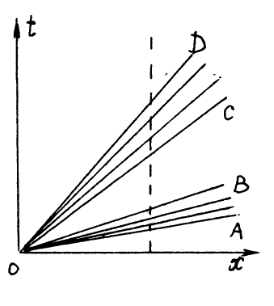
\includegraphics[width=1\linewidth]{pics/2-3-2.png}
\caption{}
\label{2-3-2}
\end{minipage}
\hfill
\begin{minipage}[h]{0.45\linewidth}
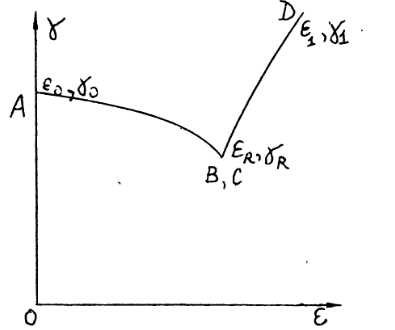
\includegraphics[width=1.1\linewidth]{pics/2-3-3.png}
\caption{}
\label{2-3-3}
\end{minipage}
\end{center}
\end{figure}
область граничных данных ($\varepsilon = \varepsilon_{1}$, $\gamma = \gamma_1$). Вдоль каждого луча $y = x/t = \const$ имеем $\varepsilon = \const$, $\gamma = \const$. В некотором сечении трубы $x = \overline{x}$ процесс деформации имеет вид, представленный на рис. \ref{2-3-3}. При движении от луча OA к лучу OB деформации изменяются по интервалу AB (рис. ref{2-3-3}) интегральной кривой уравнения \eqref{eq:2314} для $\xi = \xi_{\text{Б}}$, проходящей через точку $\varepsilon = \varepsilon_0$, $\gamma = \gamma_0$. На лучах OB и OC (рис. \ref{2-3-2}) $\varepsilon = \varepsilon_R$, $\gamma = \gamma_R$. Последовательность состояний в волне COD рис. \ref{2-3-2} дается кривой CD (рис. \ref{2-3-3}) -- интервал интегральной кривой уравнения \eqref{eq:2314} для $\xi = \xi_{\text{М}}$, проходящей через точку граничного состояния $\varepsilon = \varepsilon_1$, $\gamma = \gamma_1$.\\

\npart{III}{Экспериментальная часть}

Наиболее просто возбудить нелинейные волны сжатия-сдвига,
если по торцу предварительно закрученной трубы произвести 
продольный удар. Когда такое нагружение (только предварительное
статическое или суммарное, динамическое и статическое) вызывает
нелинейные деформации, по трубе распространяются нелинейные 
волны, в которых продольные и сдвиговые возмущения нераздельно 
связаны друг с другом.
\begin{wrapfigure}[20]{l}{0.4\linewidth} 
  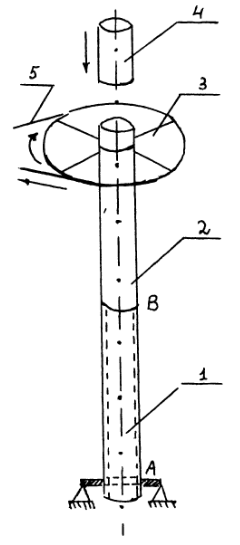
\includegraphics[width=70mm]{pics/2-3-4.png}
  \caption{}
  \label{2-3-4}
\end{wrapfigure}
Экспериментальная установка для
такого опыта состоит (рис. \ref{2-3-4}) из образца 1, передающего стержня 2 и копра 4, установленных на одной вертикальной оси. Образец -- тонкостенная труба из меди, длиной $\sim$ 500 мм, внешнего диаметре 30 мм и толщиной стенки $\sim$ 1 мм. Стержень стальной, того же диаметра и той же длины, что ж образец. В стыке B образец и стержень жестко скреплены. Нижний торец образца A удерживается от вращения шпилькой. Колесом 3, сидящим на скользящей посадке на верхней части стержня (она  эллиптического поперечного сечения), система стержень - образец статически закручивается. После этого баба копра 4 скидывается с определенней высоты и производит удар по верхнему торцу передающего стержня. В стержне возникает импульс продольной деформации. После волнового взаимодействия в стыке B в стержне возникают отраженные линейно упругие продольные и крутильные волны, а по образцу распространяются нелинейные волны сжатия-сдвига.

Все измерения производятся тензорезисторными датчиками. Для
измерения продольных деформаций применяются линейные датчики, 
наклеенные на образец вдоль его оси. Сдвиги измеряются розетками -
парой линейных датчиков, собранных на ода ой подложке под прямым
углом друг к другу, в определенном электрическом соединении - 
наклеенных так, что продольная ось образца проходит по их 
биссектрисе. Используются малобазовые датчики (база 3-5 мм), что 
практически исключает искажение формы импульса при его записи. Для
исключения сигналов от изгибных составляющих в каждом сечении
приклеена пара диаметрально противоположных линейных датчиков и
пара розеток, соединенных в соответствующей тензометрической 
схеме. Сигналы тензодатчиков в статических нагружениях измеряются
с помощью прибора ИСД-3 (измеритель статических деформаций), 
сигналы в динамических нагружениях после электрического усиления
регистрируются на экранах двухканальных осциллографов с памятью
(осциллограммы могут воспроизводиться на экране в течение суток
желательное число раз). Тензодатчики, измеряющие продольную 
деформацию и сдвиг, расположены в одном сечении (сечение 1) 
стержня (примерно на половине его длины) и в двух сечениях образца:
на расстоянии 70 мм (сечение 2) и 220 мм (сечение 3) от стыка
(рис. \ref{2-3-4}). Выбор этих сечений продиктован следующими 
обстоятельствами: 1) в непосредственной близости от стыка волновое движение искажено неодномерностью взаимодействия передающего стержня и
образца; 2) при ограниченном числе измеряемых сечений (их два)
информация об эволюции процесса более полная, если эти сечения
разнесены как можно дальше; 3) отраженные от торца A (рис. \ref{2-3-4}) волны не должны достигнуть сечения 3 раньше, чем в нем 
произойдет полная регистрация падающих волн.

Для снятия осциллограмм с каждого сечения служит свой осциллограф; на экране верхний луч отмечает возмущение $\Delta \varepsilon$, нижний -- $\Delta\gamma$.

С помощью осциллограммы в сечении 1 определяется величина $\varepsilon_i$ деформации в падающей продольной волне в стержне. Так как эта волна линейноупругая, то скорость частиц в ней равна $v_{i} = -a_{0}\varepsilon_i$, где $a_{0} = \sqrt{E_{0}/\rho_0}$ скорость упругой волны в стержне. Это и есть скорость удара по торцу образца. По этой же осциллограмме находится время нарастания импульса $t_{\text{ср}}$ и продолжительность $t_i$ его постоянной части. Величина $t_{\text{ср}}$ позволяет судить о степени приближения граничных условий к автомодельности.

Начальный сдвиг $\gamma_0$ в образце определяется с помощью тензодатчиков в сечениях 2 и 3. Близостью их показаний контролируется также однородность распределения $\gamma_0$ по длине образца. Начальная продольная деформация $\varepsilon_{0} = 0$.

Таким образом определяются граничные и начальные условия
эксперимента.

Для получения экспериментальной волновой картины в физической плоскости (рис. \ref{2-3-2}) и процесса деформации (рис. \ref{2-3-2}) по осциллограммам в сечениях 2 и 3 строятся сначала графики зависимости $\gamma(\varepsilon)$ в этих сечениях. Наклон луча ОА (рис. \ref{2-3-2}), как было проверено в других экспериментах на этой установке, равен скорости упругих волн в материале образца $a = \sqrt{E/\rho}$. Поскольку масштаб времени на осциллограммах известен, определение наклонов лучей OB (задний фронт быстрой простой волны) и ОС (передний фронт медленной волны) не представляет труда. За граничное значение $\varepsilon = \varepsilon_1$, $\gamma = \gamma_1$ принимаются те значения $\varepsilon,\ \gamma$, с которых начинается разгрузка. Они легко определяются по графикам $\gamma(\varepsilon)$: модуль радиуса-вектора в этой точке начинает резко убывать. По значению $\varepsilon_1$ (или $\gamma_1$) на осциллограмме определяется соответствующий момент времени, а затем и наклон прямой OD (рис. \ref{2-3-2}). Построение волновой картины окончено.

\npart{IV}{Обработка и анализ результатов}

В протокол задачи включается:\\
1) Краткое описание постановки эксперимента.\\
2) Геометрические и механические характеристики передающего
стержня и образца в виде таблицы.

Геометрические размеры снимаются студентами с помощью штангенциркуля. Значения $E$ и $\rho$ берутся из справочников, $a$ вычисляется.

\begin{center}
		\begin{tabular}{|c|c|c|c|c|c|c|c|}
			 \hline
			 & $\text{Материал}$ & $\text{длина, }$ & $\text{внешний}$ & $\text{толщина}$ & $E,$ & $\rho,$ & $a = $\\

			 &  & $\text{ мм}$ & $\text{диаметр,}$ & $\text{стенки}$ & $\text{МПа}$ & $\text{кг/м}^3$ & $ = \sqrt{\frac{E}{\rho}}$\\

			 & &  & $\text{мм}$ & $\text{мм}$ &  &  & $\text{м/с}$\\
			 \hline
			 $\text{образец}$&&&&&&&\\ \hline
			$\text{стержень}$&&&&&&&\\ \hline
			
		\end{tabular} 
\end{center}

3) Характеристики падающего импульса в стержне: $\varepsilon_i$, $v_i$ (м/с), $t_i$ (мкс), $t_{\text{ср}}$ (мкс).\\
4) Начальная деформация образца $\varepsilon_0$, $\gamma_0$\\
5) Графики зависимостей $\gamma(\varepsilon)$ в сечениях 2 и 3 образца. Для каждой простой волны на графике должно быть не менее 5 точек\\
6) Расчет волновой картины в сечении 3.

Масштаб времени во всех каналах всех осциллографов 25 мкс на одно (горизонтальное) деление сетки экрана осциллографа. Для перевода величины записанного на осциллографе электрического импульса $\Delta U$ (по вертикали сетки экрана) в соответствующее значение импульса деформации $\Delta \varepsilon$ (или $\Delta\gamma$) использовать формулу
\[ \Delta \varepsilon = \frac{\Delta U}{ K_{\text{П}}}\]
где $K_{\text{П}}$ -- коэффициент чувствительности тензометрической схемы. Его значение для каждого канала осциллографов дается руководителем эксперимента; при этом заполняется таблица:
\begin{center}
		\begin{tabular}{|p{3cm}|c|p{5cm}|}
			 \hline
			 \makecell{Сечения} & \makecell{Каналы осциллографов} & \makecell{$K_\text{П}$} \\ \hline

			 \multirow{2}{*}{1} & $\Delta \varepsilon$ &\\
			\cline{2-3}
             & $\Delta \gamma$ & \\ \hline

             \multirow{2}{*}{2} & $\Delta \varepsilon$ &\\
			\cline{2-3}
             & $\Delta \gamma$ & \\ \hline

             \multirow{2}{*}{3} & $\Delta \varepsilon$ &\\
			\cline{2-3}
             & $\Delta \gamma$ & \\ \hline
			
		\end{tabular} 
\end{center}

Обработка осциллограмм производится не на самом экране осциллографа, а путем оптического увеличения его изображения на фотопленке (ширина 36 мм).\\

\begin{center}
ЛИТЕРАТУРА
\end{center}

\noindent 1. Рахматулин Х.А., Демьянов Ю.А. Прочность при интенсивных кратковременных нагрузках. М.: Физматгиз, 1961.\\
2. Рахматулин Х.А. О распространении упруго-пластических волн при сложном нагружении // ПМM. 1958. Т2, вып.2. С.759-765.\\
3. Анциферов B.С., Рахматулин Х.А. Распространение сжимающе-сдвигающих возмущений в нелинейно-упругой среде // ПММ. 1964. Т.28, вып.3. С 572-578.\\
4. Ильюшин А.А. Механика сплошной среды. М.: Изд-во МГУ, 1978.\\
5. Рождественский Б.Л., Яненко Н.Н. Системы квазилинейных уравнений и их приложения к газовой динамике. М.: Наука, 1978.\\
6. Ленский Э.В. Аналитические методы динамической теории нелинейной упругости (комбинированные нелинейно-упругие волны). М.: Изд-во МГУ, 1983.

\newpage
\anonsubsection{Задача 4. Прямой экспериментальный метод построения ударных диаграмм сжатия грунтов}

Целью работы является изучение одного из методов прямого экспериментального построения динамической диаграммы сжатия грунта (песка) на основе измерения скорости распространения продольное волны сжатия в грунте при ударном нагружении.

\npart{I}{Теоретическая часть}

С помощью ударного копра в образце грунта инициируется ударная волна. Измерительная техника фиксирует время прохождения этой волны по образцу, что дает возможность вычислить скорость ударной волны. Решение соответствующей теоретической задачи позволит определить значения плотности и давления за ударном полной и по ним построить диаграмму ударного сжатия образца грунта.

\addtocounter{equation}{1}
	\begin{equation}\label{eq:241}
	 \frac{\partial^2 u}{\partial t^2} = \frac{1}{\rho_0} \frac{\partial \sigma}{\partial x},
	\tag{1}
	\end{equation} 
$\sigma = f(\varepsilon)$      $\varepsilon = \partial u / \partial x$

\addtocounter{equation}{1}
	\begin{equation}\label{eq:242}
	 \frac{\partial^2 u}{\partial t^2} = a^2(\varepsilon) \frac{\partial^2 u}{\partial x^2}, \quad \text{где} \quad a(\varepsilon) = \sqrt{\frac{1}{\rho_0} \frac{ d \sigma}{ d \varepsilon}}
	\tag{2}
	\end{equation}

$ v = \partial u/ \partial t$
\addtocounter{equation}{1}
	\begin{equation}\label{eq:243}
	 \left\{
	 	\begin{array}{l}
	 		\displaystyle \frac{\partial v}{\partial t} = a^2 \displaystyle \frac{\partial \varepsilon}{\partial x}, \\
	 		\displaystyle \frac{\partial v}{\partial x} = \displaystyle \frac{\partial \varepsilon}{\partial t},
	 	\end{array}
	 \right.
	\tag{3}
	\end{equation} 
	\[
	 \frac{\partial v}{\partial t} \pm a \frac{\partial v}{\partial x}  = \pm a \left( \frac{\partial \varepsilon}{\partial t} \pm \frac{\partial \varepsilon}{\partial x}  \right)
	\]

\addtocounter{equation}{1}
	\begin{equation}\label{eq:244}
	\left\{ 
	\begin{array}{lcl}
	 dv = a(\varepsilon) d \varepsilon & \text{вдоль линии} & dx = a(\varepsilon) dt \\
	 dv = - a(\varepsilon) d \varepsilon & \text{вдоль линии} & dx = - a(\varepsilon) dt
	 \end{array}
	 \right.
	\tag{4}
	\end{equation} 
$ dx = \pm a(\varepsilon) dt $
$ \sigma = E \varepsilon$
$c = \sqrt{E/ \rho_c}$

\addtocounter{equation}{1}
	\begin{equation}\label{eq:245}
	 \left\{
	 	\begin{array}{l}
	 		x = \pm ct + const,\\
	 		v = \pm c \varepsilon + const.
	 	\end{array}
	 \right.
	\tag{5}
	\end{equation} 

\addtocounter{equation}{1}
	\begin{equation}\label{eq:246}
	 v = \pm c \varepsilon + v_0.
	\tag{6}
	\end{equation} 

\addtocounter{equation}{1}
	\begin{equation}\label{eq:247}
	 v = \pm c \varepsilon .
	\tag{7}
	\end{equation} 

\addtocounter{equation}{1}
	\begin{equation}\label{eq:248}
	 v = \frac{v_0}{2}, \quad \varepsilon = - \frac{v_0}{2 c}
	\tag{8}
	\end{equation} 

\addtocounter{equation}{1}
	\begin{equation}\label{eq:249}
	 \left\{
	 	\begin{array}{l}
	 		\rho_a D = \rho^* (D - v^*), \\
	 		\rho_a D v^* = p^* - p_a.
	 	\end{array}
	 \right.
	\tag{9}
	\end{equation}

\addtocounter{equation}{1}
	\begin{equation}\label{eq:2410}
	 v_1 = v^*, \quad \sigma_1 = - (p^* - p_a).
	\tag{10}
	\end{equation} 

\addtocounter{equation}{1}
	\begin{equation}\label{eq:2411}
	 v_1 = c \varepsilon_1 + v_0.
	\tag{11}
	\end{equation} 

\[ 
\left\{
	\begin{array}{l}
		\rho_a D = \rho^* (D - v^*), \\
	 	\rho_a D v^* = p^* - p_a, \\
	 	-E \varepsilon_1 = p^* - p_a,\\
	 	v_1 - v_0 = c \varepsilon_1,\\
	 	v_1 = v^*,	
	\end{array}
\right.	
\]



\addtocounter{equation}{1}
	\begin{equation}\label{eq:2412}
	 	\begin{array}{l}
	 		p^* - p_a = \displaystyle \frac{\rho_c c v_0}{1 + \displaystyle \frac{\rho_c}{\rho_a} \frac{c}{D}},\\
	 		1 - \displaystyle  \frac{\rho_a}{\rho^*} = \displaystyle \frac{ \displaystyle \frac{\rho_c}{\rho_a} \frac{c v_0}{D^2}}{1+ \displaystyle \frac{\rho_c}{\rho_a} \frac{c}{D}}.
	 	\end{array}
	\tag{12}
	\end{equation}

$( 1 - \rho_a/\rho^*)$ 
$D = \Delta x/ \Delta t$
$v_0 = \sqrt{2 g h}$

\begin{center}
		\begin{tabular}{|c|c|c|c|c|c|c|c|}
			 \hline
			  № & $\Delta t$ & $h$ & $v_0$ & $v^*$ & $D$ & $\varepsilon^*$ & $p^*$\\ \hline
			  1 &&&&&&&\\ \hline
			  2 &&&&&&&\\ 
			 \hline
			
		\end{tabular} 
	\end{center}

\newpage
\anonsubsection{Задача 5. Сверхзвуковое обтекание кругового конуса}
$u = V_x(\theta), \quad v = V_y(\theta)$
$\partial v/ \partial x - \partial u / \partial y = 0$

\addtocounter{equation}{1}
	\begin{equation}\label{eq:251}
	 \frac{d v}{d u} tg \theta + 1 = 0. 
	\tag{1}
	\end{equation} 

\addtocounter{equation}{1}
  \begin{equation}\label{eq:252}
   v \frac{d^2 v}{d u^2} = 1 + \left( \frac{d v}{d u} \right)^2 - \frac{1}{a^2} \left(u + v \frac{dv}{du} \right)^2 . 
  \tag{2}
  \end{equation} 
  $u^2 + v^2$
  \[
    \frac{u^2 + v^2}{2} + \frac{a^2}{\gamma - 1} = h_0,
  \]

  \addtocounter{equation}{1}
  \begin{equation}\label{eq:253}
   \text{при} \theta = \theta_0 \frac{u}{v} = tg \theta_0, 
  \tag{3}
  \end{equation} 

  \addtocounter{equation}{1}
  \begin{equation}\label{eq:254}
   \begin{array}{l}
   u + v tg \beta = V_{\infty}, \\
   v^2 = f(u),
   \end{array}
  \tag{4}
  \end{equation} 
где 
\[v^2 = (V_{\infty} - u)^2 \frac{u - V^2_{\text{кр}}/V_{\infty}}{V^2_{\text{кр}}/V_{\infty} + \frac{2}{k +1}V_{\infty} - u }  \quad - \text{уравнение ударной поляры}\]

$\beta = \beta(M_{\infty})$

\addtocounter{equation}{1}
  \begin{equation}\label{eq:255}
   u |_{\theta = \beta} = u_1(\beta), \quad v |_{\theta = \beta} = v_1(\beta), 
  \tag{5}
  \end{equation} 

\addtocounter{equation}{1}
  \begin{equation}\label{eq:256}
   \frac{dv}{du}|_{\theta = \beta} = - ctg \beta. 
  \tag{6}
  \end{equation} 

\addtocounter{equation}{1}
  \begin{equation}\label{eq:257}
   \begin{array}{l}
   \frac{d^2 v ^*}{ du^2} = F \left( u, v, \frac{dv}{du} \right),\\
   v(u_1) = v_1,\\
   \frac{dv}{du} |_{u = u_1} = ctg \beta.
   \end{array}
  \tag{7}
  \end{equation} 

\addtocounter{equation}{1}
  \begin{equation}\label{eq:258}
   u = - v \frac{d v}{du}. 
  \tag{8}
  \end{equation}

\[
  \theta = - arctg \left[ \frac{dv}{du} \right]^{-1}, \quad u_0 < u < u_1,
\]

\[
  \theta_0 = - arctg \left[ \frac{dv}{du} \right]^{-1}_0 = arctg \frac{v_0}{u_0}
\]

\[
  \frac{u_0^2 + v_0^2}{2} + \frac{\gamma}{\gamma + 1} \frac{p_0}{\rho_0} = \frac{u_1^2 + v_1^2}{2} + \frac{\gamma}{\gamma + 1}\frac{p_1}{\rho_1},
\]

\[
  \frac{p_0}{\rho_0^{\gamma}} = \frac{p_1}{\rho_1^{\gamma}}.
\]

\[
  C_x = \frac{\iint\limits_{\sum_k}(p_0 - p_{\infty})sin \theta_0 d \sigma}{\displaystyle \frac{1}{2} \rho_{\infty} V^2_{\infty} S_m} = \frac{p_0 - p_{\infty}}{\displaystyle \frac{\gamma}{2} p_{\infty} M^2_{\infty}}
\]

\[ p_0 = p_{\text{атм}} + p_{\text{0 изб}} = p_{\text{атм}} + (n - n_0)_0k_{p_0},\]
\[ p_{\text{ст}} = p_{\text{атм}} + p_{\text{ст изб}} = p_{\text{атм}} + (n - n_0)_{\text{ст}}k_{p_{\text{ст}}},\]
где $p_{\text{атм}} = p_{\delta} + \Delta p, $

\[ 
  \frac{p_0}{p_{\text{ст}}} = \left( 1 + \frac{k-1}{2}M^2 \right)^{\displaystyle \frac{k}{k-1}},
\]

\[
  \frac{F}{F_{\text{кр}}} = \frac{\left( \displaystyle 1 + \frac{k-1}{2} M^2 \right)^{\displaystyle \frac{k+1}{2(k-1)}}}{M\left(\displaystyle  \frac{k+1}{2}\right)^{\displaystyle \frac{k+1}{2(k-1)}} },
\]
\[
  q = \frac{\rho V^2}{2} = \frac{v^2}{2} \frac{\rho}{p} p_{\text{ст}} = \frac{k}{2} p_{\text{ст}}M^2
\]

\[
  \begin{array}{l}
    C_x = \displaystyle \frac{X}{q S} =\displaystyle  \frac{(n - n_0)_x K_x}{q S}, \\
    C_y = \displaystyle \frac{Y}{q S} = \displaystyle  \frac{(n - n_0)_y K_y}{q S},\\
    m_z = \displaystyle \frac{M_z}{q S b} = \displaystyle  \frac{(n - n_0)_{mz} K_{mz}}{q S b}, \\
    m_x = \displaystyle \frac{M_x}{q S d} = \displaystyle \frac{(n - n_0)_{mx} K_{mx}}{q S d},
  \end{array} 
\]

\[
  \begin{array}{l}
    C_{x_1} = C_x cos \alpha - C_y sin \alpha,\\
    C_{y_1} = C_x sin \alpha + C_y cos \alpha, \\
    m_{z_1} = m_z, \quad m_{x_1} = m_x. 
  \end{array} 
\]

\[ m_{zA} = m_{z0b} - \frac{b_0}{b} C_{y_1}, \]

\[ C_{g} = x_{g} / b = m_{zA}/C_{y_1}  \]
\anonsubsection{Задача 6. Соударение двух упругих тел}

\anonsubsection{Задача 7. Экспериментальное исследование подводного взрыва сферического заряда}
\anonsubsection{Задача 8. Влияние вращения цилиндра, находящегося в поперечном потоке, на распределение давления по его поверхности}


\end{document}
